% Options for packages loaded elsewhere
\PassOptionsToPackage{unicode}{hyperref}
\PassOptionsToPackage{hyphens}{url}
%
\documentclass[
  10pt,
  ignorenonframetext,
]{beamer}
\usepackage{pgfpages}
\setbeamertemplate{caption}[numbered]
\setbeamertemplate{caption label separator}{: }
\setbeamercolor{caption name}{fg=normal text.fg}
\beamertemplatenavigationsymbolsempty
% Prevent slide breaks in the middle of a paragraph
\widowpenalties 1 10000
\raggedbottom
\setbeamertemplate{part page}{
  \centering
  \begin{beamercolorbox}[sep=16pt,center]{part title}
    \usebeamerfont{part title}\insertpart\par
  \end{beamercolorbox}
}
\setbeamertemplate{section page}{
  \centering
  \begin{beamercolorbox}[sep=12pt,center]{part title}
    \usebeamerfont{section title}\insertsection\par
  \end{beamercolorbox}
}
\setbeamertemplate{subsection page}{
  \centering
  \begin{beamercolorbox}[sep=8pt,center]{part title}
    \usebeamerfont{subsection title}\insertsubsection\par
  \end{beamercolorbox}
}
\AtBeginPart{
  \frame{\partpage}
}
\AtBeginSection{
  \ifbibliography
  \else
    \frame{\sectionpage}
  \fi
}
\AtBeginSubsection{
  \frame{\subsectionpage}
}
\usepackage{amsmath,amssymb}
\usepackage{iftex}
\ifPDFTeX
  \usepackage[T1]{fontenc}
  \usepackage[utf8]{inputenc}
  \usepackage{textcomp} % provide euro and other symbols
\else % if luatex or xetex
  \usepackage{unicode-math} % this also loads fontspec
  \defaultfontfeatures{Scale=MatchLowercase}
  \defaultfontfeatures[\rmfamily]{Ligatures=TeX,Scale=1}
\fi
\usepackage{lmodern}
\usetheme[]{Berlin}
\usecolortheme{dolphin}
\usefonttheme{serif} % use mainfont rather than sansfont for slide text
\ifPDFTeX\else
  % xetex/luatex font selection
  \setmainfont[]{Calibri}
  \setsansfont[]{Calibri}
  \setmonofont[]{Consolas}
\fi
% Use upquote if available, for straight quotes in verbatim environments
\IfFileExists{upquote.sty}{\usepackage{upquote}}{}
\IfFileExists{microtype.sty}{% use microtype if available
  \usepackage[]{microtype}
  \UseMicrotypeSet[protrusion]{basicmath} % disable protrusion for tt fonts
}{}
\makeatletter
\@ifundefined{KOMAClassName}{% if non-KOMA class
  \IfFileExists{parskip.sty}{%
    \usepackage{parskip}
  }{% else
    \setlength{\parindent}{0pt}
    \setlength{\parskip}{6pt plus 2pt minus 1pt}}
}{% if KOMA class
  \KOMAoptions{parskip=half}}
\makeatother
\usepackage{xcolor}
\newif\ifbibliography
\usepackage{color}
\usepackage{fancyvrb}
\newcommand{\VerbBar}{|}
\newcommand{\VERB}{\Verb[commandchars=\\\{\}]}
\DefineVerbatimEnvironment{Highlighting}{Verbatim}{commandchars=\\\{\}}
% Add ',fontsize=\small' for more characters per line
\usepackage{framed}
\definecolor{shadecolor}{RGB}{248,248,248}
\newenvironment{Shaded}{\begin{snugshade}}{\end{snugshade}}
\newcommand{\AlertTok}[1]{\textcolor[rgb]{0.94,0.16,0.16}{#1}}
\newcommand{\AnnotationTok}[1]{\textcolor[rgb]{0.56,0.35,0.01}{\textbf{\textit{#1}}}}
\newcommand{\AttributeTok}[1]{\textcolor[rgb]{0.13,0.29,0.53}{#1}}
\newcommand{\BaseNTok}[1]{\textcolor[rgb]{0.00,0.00,0.81}{#1}}
\newcommand{\BuiltInTok}[1]{#1}
\newcommand{\CharTok}[1]{\textcolor[rgb]{0.31,0.60,0.02}{#1}}
\newcommand{\CommentTok}[1]{\textcolor[rgb]{0.56,0.35,0.01}{\textit{#1}}}
\newcommand{\CommentVarTok}[1]{\textcolor[rgb]{0.56,0.35,0.01}{\textbf{\textit{#1}}}}
\newcommand{\ConstantTok}[1]{\textcolor[rgb]{0.56,0.35,0.01}{#1}}
\newcommand{\ControlFlowTok}[1]{\textcolor[rgb]{0.13,0.29,0.53}{\textbf{#1}}}
\newcommand{\DataTypeTok}[1]{\textcolor[rgb]{0.13,0.29,0.53}{#1}}
\newcommand{\DecValTok}[1]{\textcolor[rgb]{0.00,0.00,0.81}{#1}}
\newcommand{\DocumentationTok}[1]{\textcolor[rgb]{0.56,0.35,0.01}{\textbf{\textit{#1}}}}
\newcommand{\ErrorTok}[1]{\textcolor[rgb]{0.64,0.00,0.00}{\textbf{#1}}}
\newcommand{\ExtensionTok}[1]{#1}
\newcommand{\FloatTok}[1]{\textcolor[rgb]{0.00,0.00,0.81}{#1}}
\newcommand{\FunctionTok}[1]{\textcolor[rgb]{0.13,0.29,0.53}{\textbf{#1}}}
\newcommand{\ImportTok}[1]{#1}
\newcommand{\InformationTok}[1]{\textcolor[rgb]{0.56,0.35,0.01}{\textbf{\textit{#1}}}}
\newcommand{\KeywordTok}[1]{\textcolor[rgb]{0.13,0.29,0.53}{\textbf{#1}}}
\newcommand{\NormalTok}[1]{#1}
\newcommand{\OperatorTok}[1]{\textcolor[rgb]{0.81,0.36,0.00}{\textbf{#1}}}
\newcommand{\OtherTok}[1]{\textcolor[rgb]{0.56,0.35,0.01}{#1}}
\newcommand{\PreprocessorTok}[1]{\textcolor[rgb]{0.56,0.35,0.01}{\textit{#1}}}
\newcommand{\RegionMarkerTok}[1]{#1}
\newcommand{\SpecialCharTok}[1]{\textcolor[rgb]{0.81,0.36,0.00}{\textbf{#1}}}
\newcommand{\SpecialStringTok}[1]{\textcolor[rgb]{0.31,0.60,0.02}{#1}}
\newcommand{\StringTok}[1]{\textcolor[rgb]{0.31,0.60,0.02}{#1}}
\newcommand{\VariableTok}[1]{\textcolor[rgb]{0.00,0.00,0.00}{#1}}
\newcommand{\VerbatimStringTok}[1]{\textcolor[rgb]{0.31,0.60,0.02}{#1}}
\newcommand{\WarningTok}[1]{\textcolor[rgb]{0.56,0.35,0.01}{\textbf{\textit{#1}}}}
\usepackage{graphicx}
\makeatletter
\def\maxwidth{\ifdim\Gin@nat@width>\linewidth\linewidth\else\Gin@nat@width\fi}
\def\maxheight{\ifdim\Gin@nat@height>\textheight\textheight\else\Gin@nat@height\fi}
\makeatother
% Scale images if necessary, so that they will not overflow the page
% margins by default, and it is still possible to overwrite the defaults
% using explicit options in \includegraphics[width, height, ...]{}
\setkeys{Gin}{width=\maxwidth,height=\maxheight,keepaspectratio}
% Set default figure placement to htbp
\makeatletter
\def\fps@figure{htbp}
\makeatother
\setlength{\emergencystretch}{3em} % prevent overfull lines
\providecommand{\tightlist}{%
  \setlength{\itemsep}{0pt}\setlength{\parskip}{0pt}}
\setcounter{secnumdepth}{-\maxdimen} % remove section numbering
% ----------------------------
% Fonts
% ----------------------------
\usepackage{fontspec}
\setmainfont{Calibri}
\setsansfont{Calibri}
\setmonofont{Consolas}
\renewcommand{\familydefault}{\sfdefault}

% ----------------------------
% Packages usuels
% ----------------------------
\usepackage{amssymb,amsmath,amsthm,enumerate}
\usepackage{array}
\usepackage{parskip}
\usepackage{graphicx}
\usepackage{caption}
\captionsetup[figure]{labelformat=empty}
\usepackage{subcaption}
\usepackage{bm}
\usepackage{multicol}
\usepackage{tcolorbox}
\usepackage{siunitx}
\usepackage{booktabs}

% ----------------------------
% Beamer navigation
% ----------------------------
% Supprimer les icônes en bas
\setbeamertemplate{navigation symbols}{}

% Activer les mini-frames (petits ronds)
\useoutertheme{miniframes}

% Section en gras dans la barre du haut
\setbeamerfont{section in head/foot}{series=\bfseries}

% ----------------------------
% Headline sur 2 lignes :
% 1) Sections (en haut)
% 2) Mini-frames seuls (en dessous)
% ----------------------------
\makeatletter
\setbeamertemplate{headline}{%
  % --- Ligne 1 : sections
  \begin{beamercolorbox}[wd=\paperwidth,ht=2.8ex,dp=1.2ex]{section in head/foot}%
    \insertsectionnavigationhorizontal{\paperwidth}{}{}%
  \end{beamercolorbox}%
}
\makeatother

% ----------------------------
% (Optionnel) : pas de barre sur la slide de titre
% ----------------------------
\addtobeamertemplate{title page}{\setbeamertemplate{headline}{}}{}

\ifLuaTeX
  \usepackage{selnolig}  % disable illegal ligatures
\fi
\usepackage{bookmark}
\IfFileExists{xurl.sty}{\usepackage{xurl}}{} % add URL line breaks if available
\urlstyle{same}
\hypersetup{
  pdftitle={R pour jeunes économistes},
  pdfauthor={J.-B. Guiffard},
  hidelinks,
  pdfcreator={LaTeX via pandoc}}

\title{R pour jeunes économistes}
\subtitle{Manipuler des données cartographique sur R}
\author{J.-B. Guiffard}
\date{22 mai 2026}

\begin{document}
\frame{\titlepage}

\section{Données spatiales et cartes avec
R}\label{donnuxe9es-spatiales-et-cartes-avec-r}

\begin{frame}{Objet de la séance}
\phantomsection\label{objet-de-la-suxe9ance}
Cette séance est consacrée à l'utilisation de R pour manipuler, analyser
et représenter des données spatiales.

L'objectif est de comprendre comment passer :

\[
\text{données géographiques}
\rightarrow
\text{base spatiale}
\rightarrow
\text{carte}
\rightarrow
\text{variable d’analyse}
\]

Nous verrons comment utiliser R pour :

\begin{itemize}
\tightlist
\item
  lire des fichiers cartographiques ;
\item
  manipuler des objets spatiaux ;
\item
  produire des cartes ;
\item
  joindre des données statistiques à des géométries ;
\item
  calculer des distances et des intersections ;
\item
  introduire les données raster.
\end{itemize}
\end{frame}

\begin{frame}{Pourquoi spatialiser les données ?}
\phantomsection\label{pourquoi-spatialiser-les-donnuxe9es}
De nombreuses questions en économie appliquée ont une dimension
spatiale.

Exemples :

\begin{itemize}
  \item accès aux infrastructures ;
  \item exposition au climat ou à la pollution ;
  \item distance aux marchés, aux routes ou aux services publics ;
  \item inégalités territoriales ;
  \item localisation des entreprises, écoles ou ménages ;
  \item diffusion spatiale d’un traitement ou d’une politique publique.
\end{itemize}

\(\Rightarrow\) Spatialiser les données permet de relier des phénomènes
économiques à des lieux, des distances et des territoires.
\end{frame}

\begin{frame}[fragile]{Plan de la séance}
\phantomsection\label{plan-de-la-suxe9ance}
\begin{enumerate}
\tightlist
\item
  Comprendre les principaux types de données spatiales
\item
  Lire et manipuler des données vectorielles avec \texttt{sf}
\item
  Produire des cartes avec \texttt{ggplot2}, \texttt{tmap} et
  \texttt{mapview}
\item
  Joindre des données socio-économiques à des données géographiques
\item
  Manipuler des points, des distances et des rasters
\end{enumerate}
\end{frame}

\section{Pourquoi les données spatiales en économie
?}\label{pourquoi-les-donnuxe9es-spatiales-en-uxe9conomie}

\begin{frame}{Pourquoi spatialiser les données ?}
\phantomsection\label{pourquoi-spatialiser-les-donnuxe9es-1}
De nombreuses questions en économie appliquée ont une dimension
spatiale.

Les phénomènes économiques ne se distribuent pas de manière uniforme
dans l'espace :

\begin{itemize}
  \item les infrastructures sont localisées ;
  \item les ménages et les entreprises sont situés à des endroits précis ;
  \item les politiques publiques peuvent cibler certains territoires ;
  \item les conditions climatiques varient selon les lieux ;
  \item l’accès aux marchés, aux écoles ou aux services publics dépend de la distance.
\end{itemize}
\end{frame}

\begin{frame}{Quelques exemples de questions de recherche}
\phantomsection\label{quelques-exemples-de-questions-de-recherche}
Les données spatiales peuvent être utiles dans de nombreux champs de
l'économie.

\begin{itemize}
  \item Quel est l’effet de l’accès à une route sur l’activité économique locale ?
  \item Les écoles connectées à Internet obtiennent-elles de meilleurs résultats ?
  \item Comment l’exposition à la sécheresse affecte-t-elle les revenus agricoles ?
  \item Les entreprises proches d’une infrastructure numérique deviennent-elles plus productives ?
  \item Les ménages éloignés des services publics sont-ils moins bien couverts ?
  \item Comment les politiques publiques se diffusent-elles entre territoires voisins ?
\end{itemize}
\end{frame}

\begin{frame}{Trois usages des données spatiales}
\phantomsection\label{trois-usages-des-donnuxe9es-spatiales}
Dans un projet empirique, les données spatiales peuvent servir à
plusieurs choses.

\begin{enumerate}
  \item \textbf{Décrire} : représenter la distribution spatiale d’un phénomène.
  \item \textbf{Construire des variables} : distance, exposition, accessibilité, appartenance à une zone.
  \item \textbf{Analyser} : étudier les inégalités territoriales, les effets de voisinage ou l’impact d’une politique localisée.
\end{enumerate}

Exemples :

\begin{itemize}
  \item distance à une route, un port ou une capitale ;
  \item exposition à une température ou une sécheresse ;
  \item nombre d’écoles dans une commune ;
  \item appartenance à une zone traitée.
\end{itemize}
\end{frame}

\begin{frame}{Exemple 1 : infrastructures et développement}
\phantomsection\label{exemple-1-infrastructures-et-duxe9veloppement}
Supposons que l'on étudie l'effet d'une nouvelle route, d'un câble
Internet ou d'une ligne électrique.

Les données spatiales permettent de construire plusieurs variables :

\begin{itemize}
  \item distance à l’infrastructure ;
  \item présence de l’infrastructure dans une zone ;
  \item date d’arrivée de l’infrastructure ;
  \item nombre d’infrastructures autour d’un lieu ;
  \item exposition différenciée selon la proximité.
\end{itemize}

Ces variables peuvent ensuite être utilisées dans une analyse
économétrique.

Ex : Comparer les zones proches et éloignées d'une infrastructure avant
et après son déploiement.
\end{frame}

\begin{frame}{Exemple 1 : infrastructures et développement}
\phantomsection\label{exemple-1-infrastructures-et-duxe9veloppement-1}
\centering

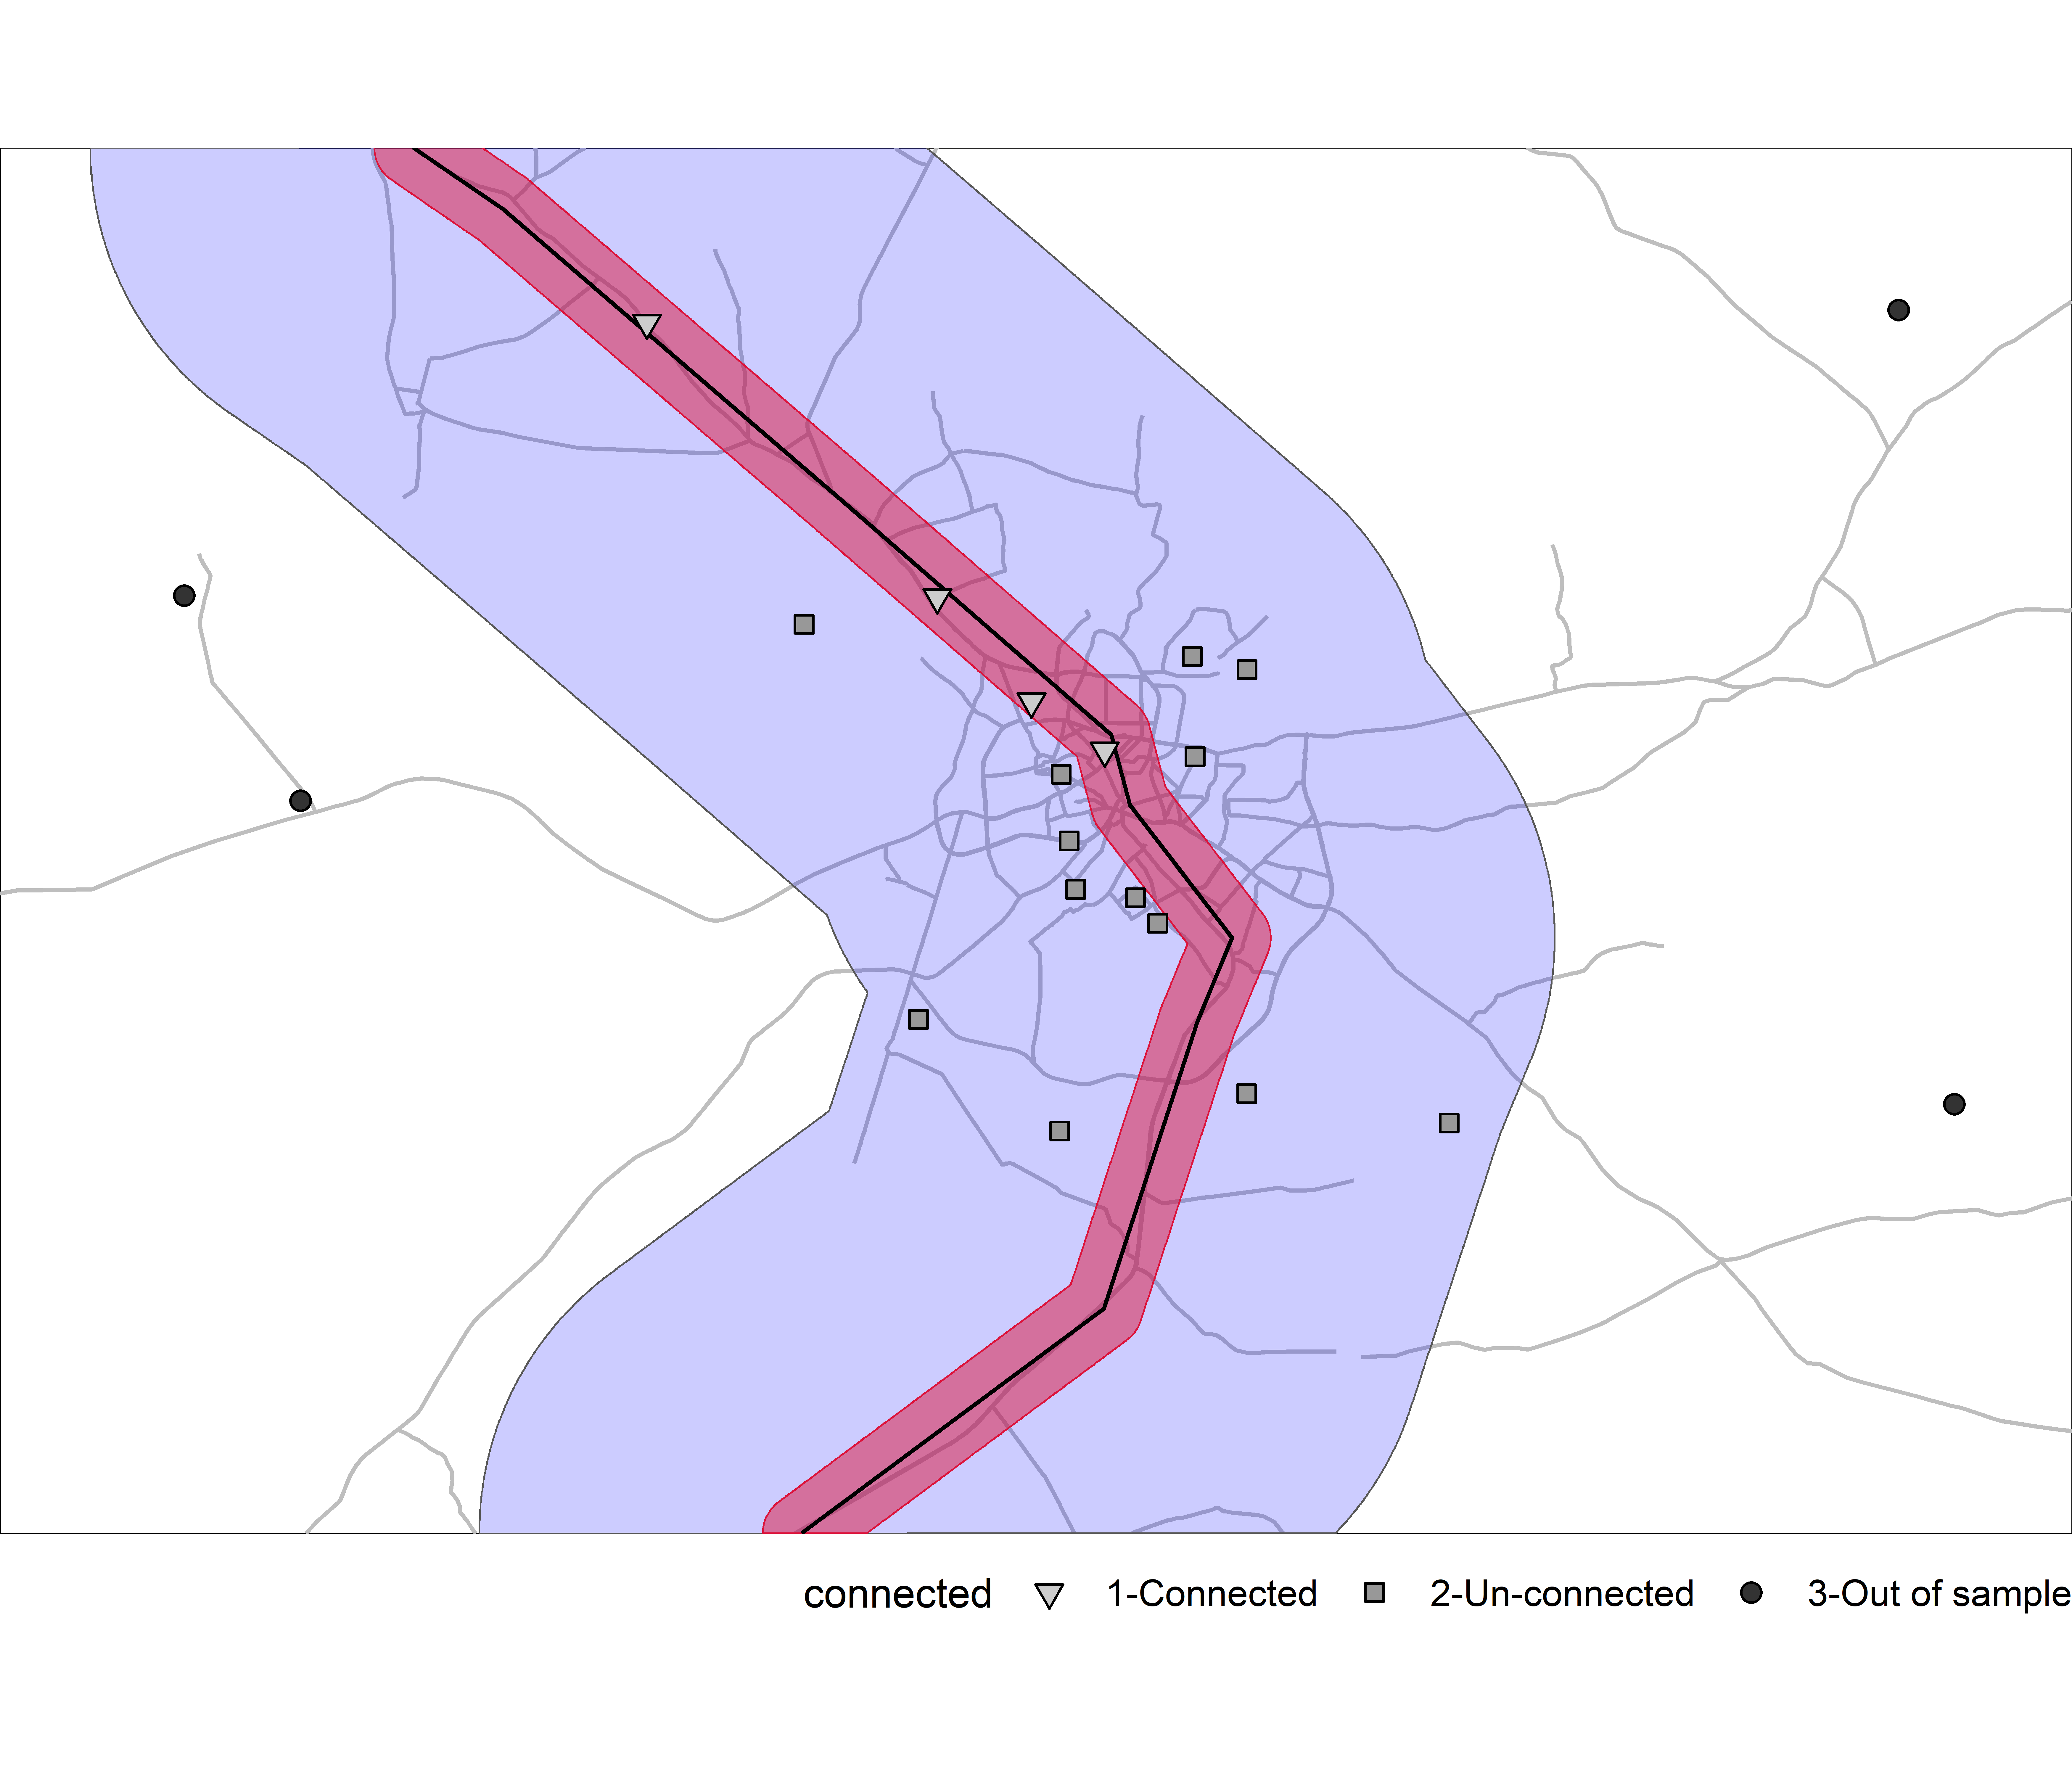
\includegraphics{figures/carte_ex_1.png}
\end{frame}

\begin{frame}{Exemple 2 : climat, agriculture et revenus}
\phantomsection\label{exemple-2-climat-agriculture-et-revenus}
Les données climatiques sont souvent disponibles sous forme de grilles
spatiales.

Chaque pixel peut contenir une information :

\begin{itemize}
  \item température ;
  \item précipitations ;
  \item sécheresse ;
  \item humidité des sols ;
  \item végétation ;
  \item altitude.
\end{itemize}
\end{frame}

\begin{frame}{Exemple 2}
\phantomsection\label{exemple-2}
On peut ensuite associer ces informations à des unités économiques :

\begin{itemize}
  \item ménages ;
  \item exploitations agricoles ;
  \item communes ;
  \item régions ;
  \item pays.
\end{itemize}

Question empirique : Comment l'exposition à un choc climatique
affecte-t-elle les revenus, les migrations ou la production agricole ?
\end{frame}

\begin{frame}{Exemple 2}
\phantomsection\label{exemple-2-1}
\centering

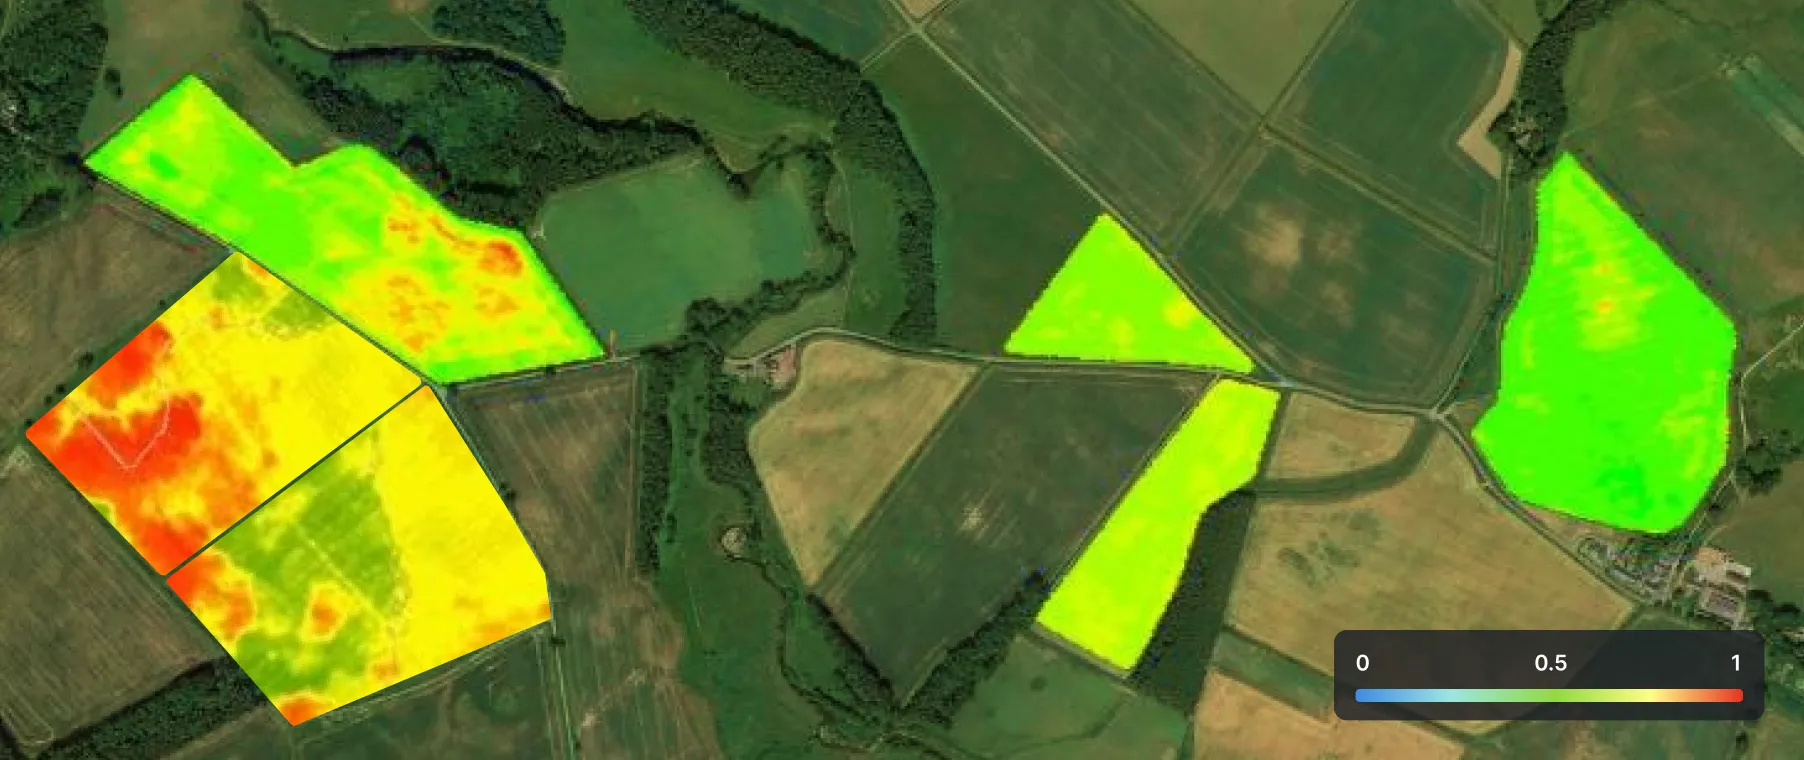
\includegraphics{figures/ndvi.png}
\end{frame}

\begin{frame}{Exemple 3 : services publics et accessibilité}
\phantomsection\label{exemple-3-services-publics-et-accessibilituxe9}
L'accès aux services publics dépend souvent de la localisation.

On peut étudier par exemple :

\begin{itemize}
  \item la distance à l’école la plus proche ;
  \item la distance à un centre de santé ;
  \item le temps d’accès à une route ;
  \item la couverture d’un réseau mobile ;
  \item la proximité d’une administration publique.
\end{itemize}

Ces mesures permettent de construire des indicateurs d'accessibilité.
\end{frame}

\begin{frame}{Exemple 4 : politiques publiques localisées}
\phantomsection\label{exemple-4-politiques-publiques-localisuxe9es}
Certaines politiques publiques ne s'appliquent pas partout de la même
manière.

Elles peuvent cibler :

\begin{itemize}
  \item certaines communes ;
  \item certaines écoles ;
  \item certaines régions ;
  \item certaines zones frontalières ;
  \item certaines zones exposées à un risque.
\end{itemize}
\end{frame}

\begin{frame}{Exemple 4}
\phantomsection\label{exemple-4}
Les données spatiales permettent alors de définir :

\begin{itemize}
  \item les zones traitées ;
  \item les zones de comparaison ;
  \item les distances aux frontières du traitement ;
  \item les unités exposées indirectement.
\end{itemize}

La localisation peut aider à définir un traitement, une exposition ou un
groupe de contrôle.
\end{frame}

\begin{frame}{Exemple 4}
\phantomsection\label{exemple-4-1}
\centering

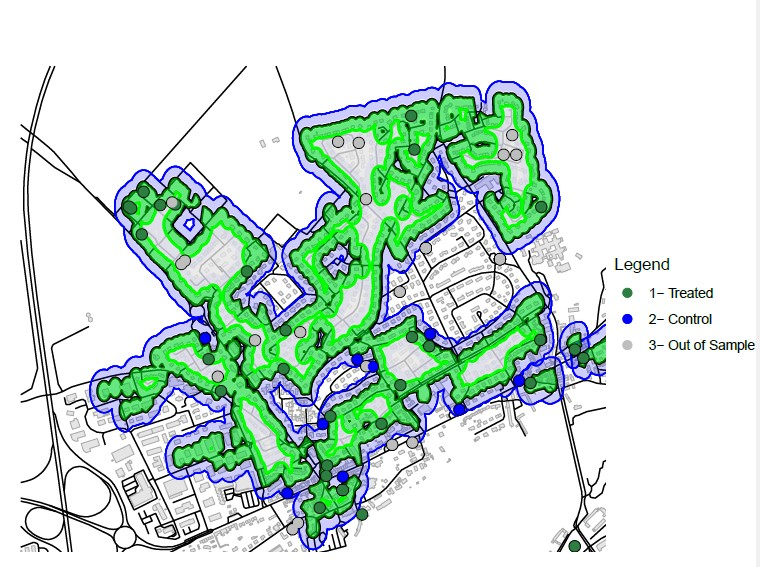
\includegraphics{figures/map_pp.jpg}
\end{frame}

\begin{frame}{Carte descriptive ou variable empirique ?}
\phantomsection\label{carte-descriptive-ou-variable-empirique}
Une carte peut avoir deux fonctions différentes.

\begin{enumerate}
  \item \textbf{Illustrer un phénomène}  
  \begin{itemize}
    \item carte du revenu par région ;
    \item carte des émissions de CO₂ par pays ;
    \item carte de la densité de population.
  \end{itemize}

  \item \textbf{Construire une variable d’analyse}  
  \begin{itemize}
    \item distance à une infrastructure ;
    \item exposition à un choc climatique ;
    \item nombre d’écoles dans une zone ;
    \item appartenance à une zone traitée.
  \end{itemize}
\end{enumerate}
\end{frame}

\begin{frame}{Ce que nous allons apprendre à faire}
\phantomsection\label{ce-que-nous-allons-apprendre-uxe0-faire}
Dans cette séance, nous allons voir comment utiliser R pour :

\begin{itemize}
  \item lire une carte sous forme de fichier spatial ;
  \item comprendre la structure d’un objet spatial ;
  \item vérifier un système de coordonnées ;
  \item joindre une base statistique à une carte ;
  \item produire une carte thématique ;
  \item manipuler des points et des polygones ;
  \item calculer des distances ou des intersections ;
  \item introduire les données raster.
\end{itemize}
\end{frame}

\section{Comprendre les objets
spatiaux}\label{comprendre-les-objets-spatiaux}

\begin{frame}{Qu'est-ce qu'une donnée spatiale ?}
\phantomsection\label{quest-ce-quune-donnuxe9e-spatiale}
Une donnée spatiale est une donnée associée à une localisation.

Elle contient généralement deux types d'information :

\begin{itemize}
  \item une information \textbf{attributaire} : nom, population, revenu, émission, statut ;
  \item une information \textbf{géographique} : coordonnées, forme, position, surface.
\end{itemize}

Exemples :

\begin{itemize}
  \item une école avec sa latitude et sa longitude ;
  \item une commune avec ses frontières ;
  \item une route avec son tracé ;
  \item une grille climatique avec une température par pixel.
\end{itemize}

Une donnée spatiale est une donnée classique à laquelle on ajoute une
dimension géographique.
\end{frame}

\begin{frame}{Les grandes familles de données spatiales}
\phantomsection\label{les-grandes-familles-de-donnuxe9es-spatiales}
On distingue principalement deux grands types de données spatiales.

\begin{enumerate}
  \item \textbf{Données vectorielles}
  \begin{itemize}
    \item points ;
    \item lignes ;
    \item polygones.
  \end{itemize}

  \item \textbf{Données raster}
  \begin{itemize}
    \item grille de pixels ;
    \item une valeur associée à chaque cellule ;
    \item utile pour les phénomènes continus.
  \end{itemize}
\end{enumerate}
\end{frame}

\begin{frame}{Les données vectorielles}
\phantomsection\label{les-donnuxe9es-vectorielles}
Les données vectorielles représentent des objets géographiques précis.

Elles peuvent prendre plusieurs formes :

\begin{itemize}
  \item \textbf{points} : écoles, entreprises, ménages, antennes, centrales ;
  \item \textbf{lignes} : routes, chemins de fer, rivières, câbles ;
  \item \textbf{polygones} : pays, régions, communes, zones administratives.
\end{itemize}

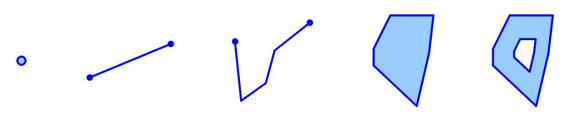
\includegraphics{figures/Vecteur.png}
\end{frame}

\begin{frame}{Les données vectorielles}
\phantomsection\label{les-donnuxe9es-vectorielles-1}
Exemples en économie appliquée :

\begin{itemize}
  \item distance d’un ménage à une route ;
  \item nombre d’écoles dans une commune ;
  \item exposition d’une entreprise à une zone traitée.
\end{itemize}
\end{frame}

\begin{frame}{Les données raster}
\phantomsection\label{les-donnuxe9es-raster}
Les données raster sont organisées sous forme de grille.

Chaque cellule ou pixel contient une valeur.

Exemples :

\begin{itemize}
  \item température ;
  \item précipitations ;
  \item altitude ;
  \item luminosité nocturne ;
  \item occupation des sols ;
  \item indice de végétation.
\end{itemize}

Ces données sont très utilisées pour mesurer des phénomènes continus
dans l'espace.

Ex : On peut calculer la température moyenne observée dans chaque
commune à partir d'un raster climatique.
\end{frame}

\begin{frame}{Les données raster}
\phantomsection\label{les-donnuxe9es-raster-1}
\centering

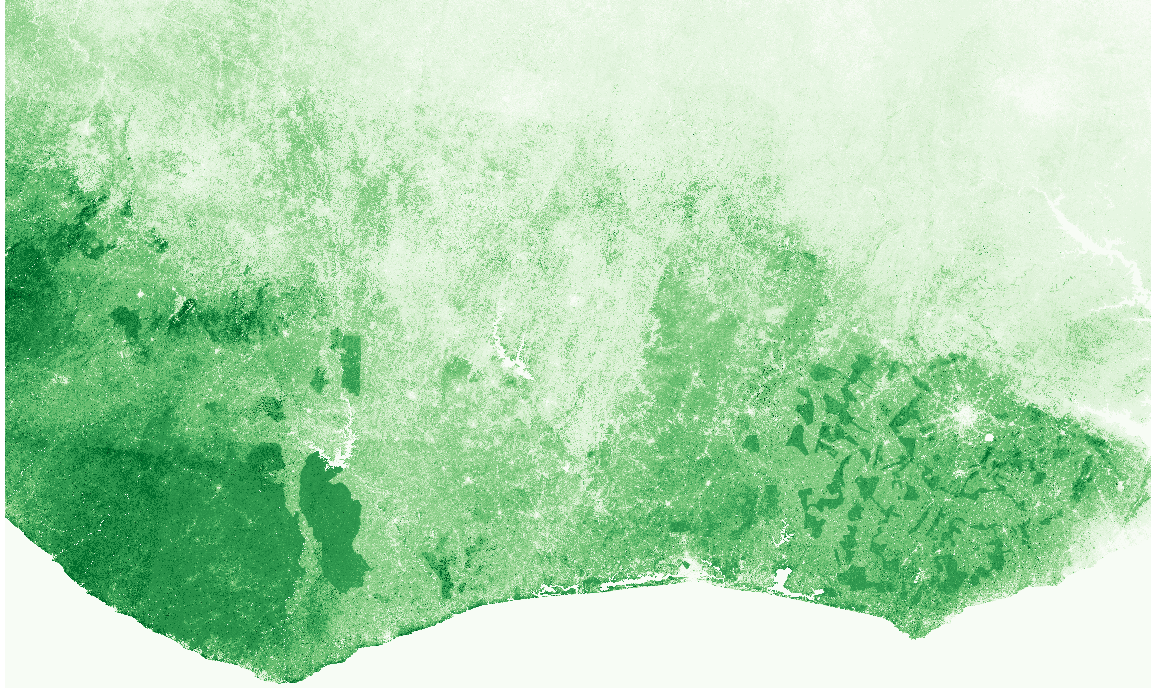
\includegraphics{figures/Raster.png}
\end{frame}

\begin{frame}{Points, polygones et rasters : exemples}
\phantomsection\label{points-polygones-et-rasters-exemples}
Une même question de recherche peut combiner plusieurs types de données.

Exemple : étudier l'effet des infrastructures scolaires sur les
résultats éducatifs.

\begin{itemize}
  \item \textbf{Points} : localisation des écoles ;
  \item \textbf{Polygones} : communes ou districts scolaires ;
  \item \textbf{Rasters} : densité de population ou accessibilité routière.
\end{itemize}

On peut ensuite construire des variables :

\begin{itemize}
  \item nombre d’écoles par commune ;
  \item distance à l’école la plus proche ;
  \item population exposée dans un rayon donné.
\end{itemize}
\end{frame}

\begin{frame}{Coordonnées géographiques}
\phantomsection\label{coordonnuxe9es-guxe9ographiques}
Pour localiser un point sur la Terre, on utilise souvent deux
coordonnées :

\[
\text{longitude}, \text{latitude}
\]

\begin{itemize}
  \item la \textbf{longitude} indique la position est-ouest ;
  \item la \textbf{latitude} indique la position nord-sud.
\end{itemize}

Exemple :

\[
\text{Paris} \approx 2.35^\circ, 48.85^\circ
\]

Attention : Les coordonnées en longitude-latitude sont exprimées en
degrés, pas en mètres.
\end{frame}

\begin{frame}{CRS : système de coordonnées}
\phantomsection\label{crs-systuxe8me-de-coordonnuxe9es}
Un CRS indique comment les coordonnées géographiques doivent être
interprétées. CRS signifie Coordinate Reference System

Il définit notamment :

\begin{itemize}
  \item le système de référence utilisé ;
  \item l’unité des coordonnées ;
  \item la manière de représenter la Terre ;
  \item la projection éventuelle utilisée.
\end{itemize}

Exemples fréquents :

\begin{itemize}
  \item \texttt{EPSG:4326} : coordonnées longitude-latitude, souvent utilisé par le GPS ;
  \item \texttt{EPSG:3857} : projection souvent utilisée pour les cartes web ;
  \item \texttt{EPSG:2154} : Lambert-93, souvent utilisé pour la France.
\end{itemize}

Avant toute opération spatiale, vérifier le CRS des données.
\end{frame}

\begin{frame}{Pourquoi les projections comptent ?}
\phantomsection\label{pourquoi-les-projections-comptent}
La Terre est une surface courbe.

Une carte est une représentation plane de cette surface.

Passer d'un globe à une carte implique donc toujours des déformations :

\begin{itemize}
  \item des surfaces ;
  \item des formes ;
  \item des distances ;
  \item des angles.
\end{itemize}

Aucune projection n'est parfaite : le choix dépend de l'usage.

Le bon système de projection dépend de ce que l'on veut faire :
afficher, mesurer une distance, calculer une surface ou comparer des
territoires.
\end{frame}

\begin{frame}{}
\phantomsection\label{section}
\centering

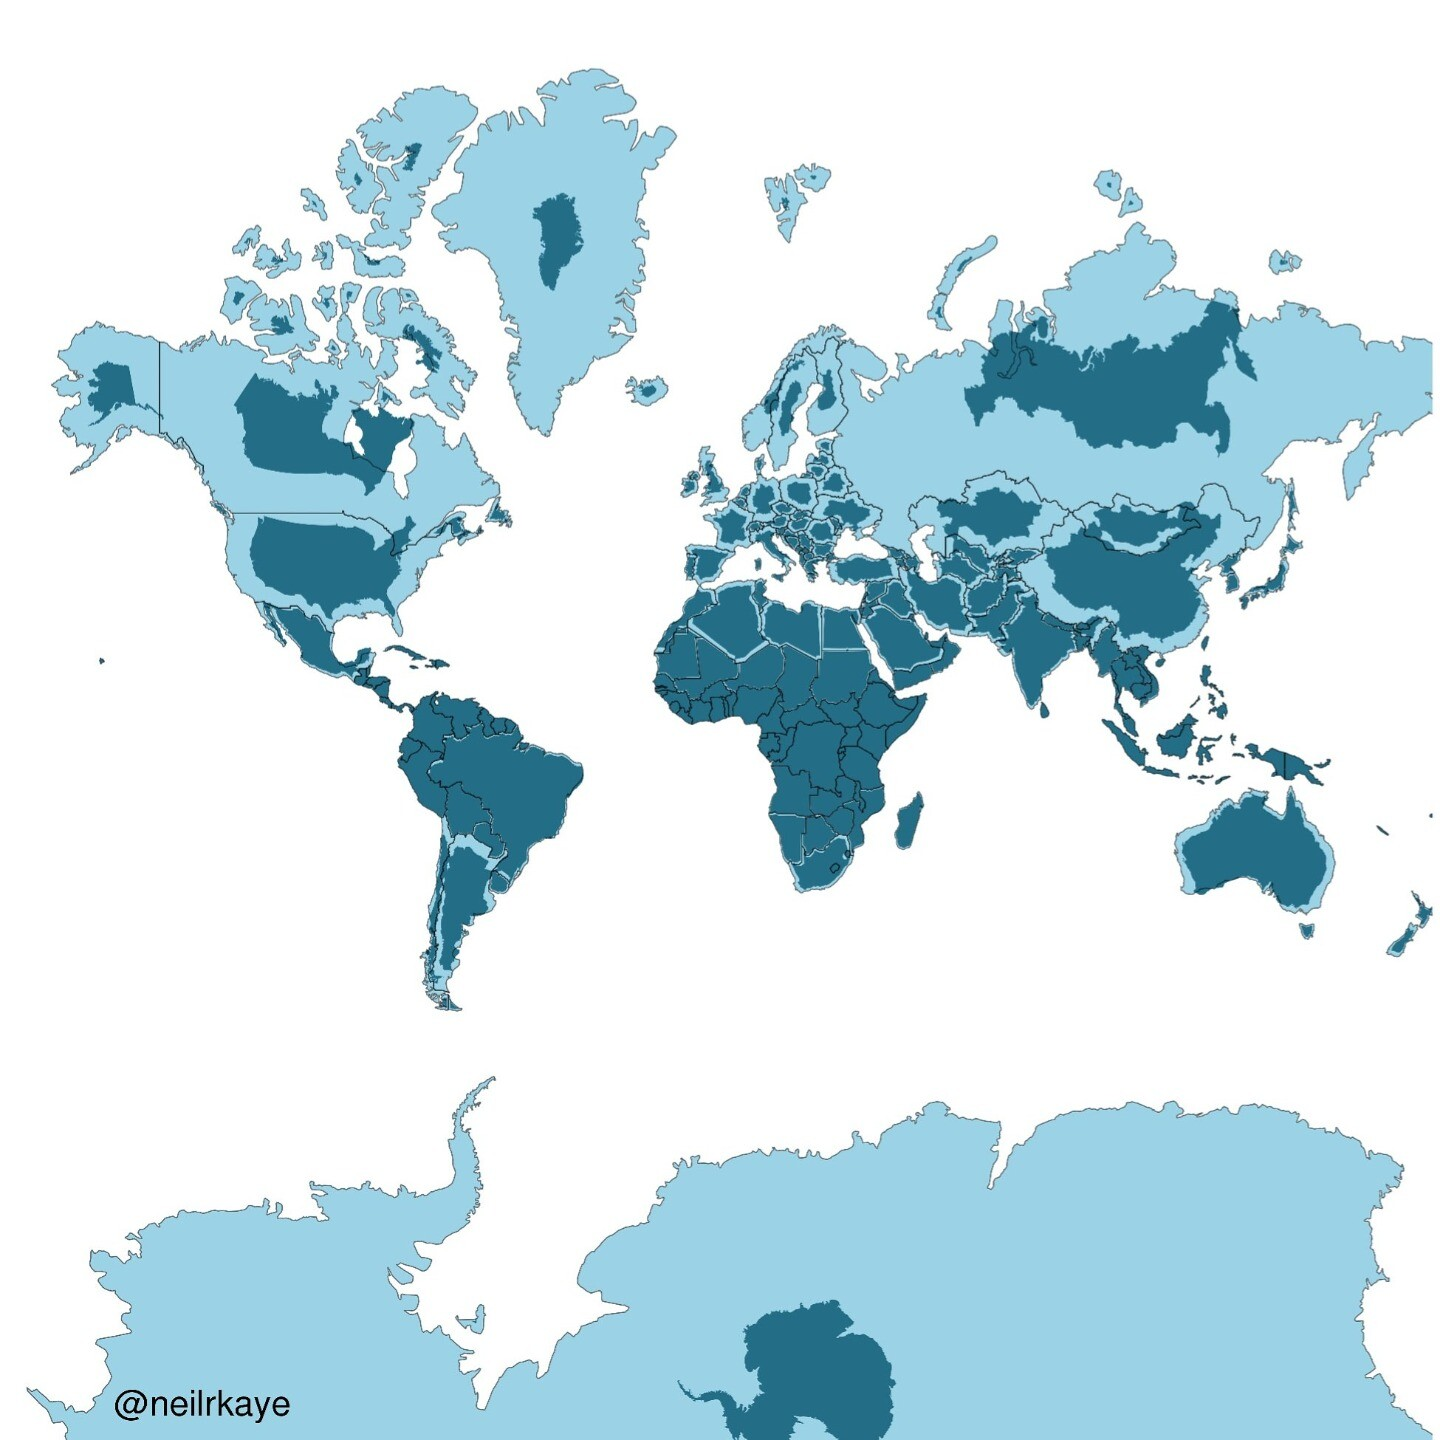
\includegraphics{figures/Mercator size vs true country size Neil Kaye.jpeg}
\end{frame}

\begin{frame}{Projection et calcul de distance}
\phantomsection\label{projection-et-calcul-de-distance}
Les calculs de distance sont sensibles au système de coordonnées.

Si les données sont en longitude-latitude :

\[
\text{les coordonnées sont en degrés}
\]

Si les données sont projetées :

\[
\text{les coordonnées peuvent être en mètres}
\]

Pour calculer des distances locales, il est souvent préférable
d'utiliser une projection adaptée.

Ex : Pour travailler sur la France métropolitaine, on utilise souvent le
Lambert-93 : EPSG:2154.
\end{frame}

\begin{frame}{Projection et calcul de distance}
\phantomsection\label{projection-et-calcul-de-distance-1}
\centering

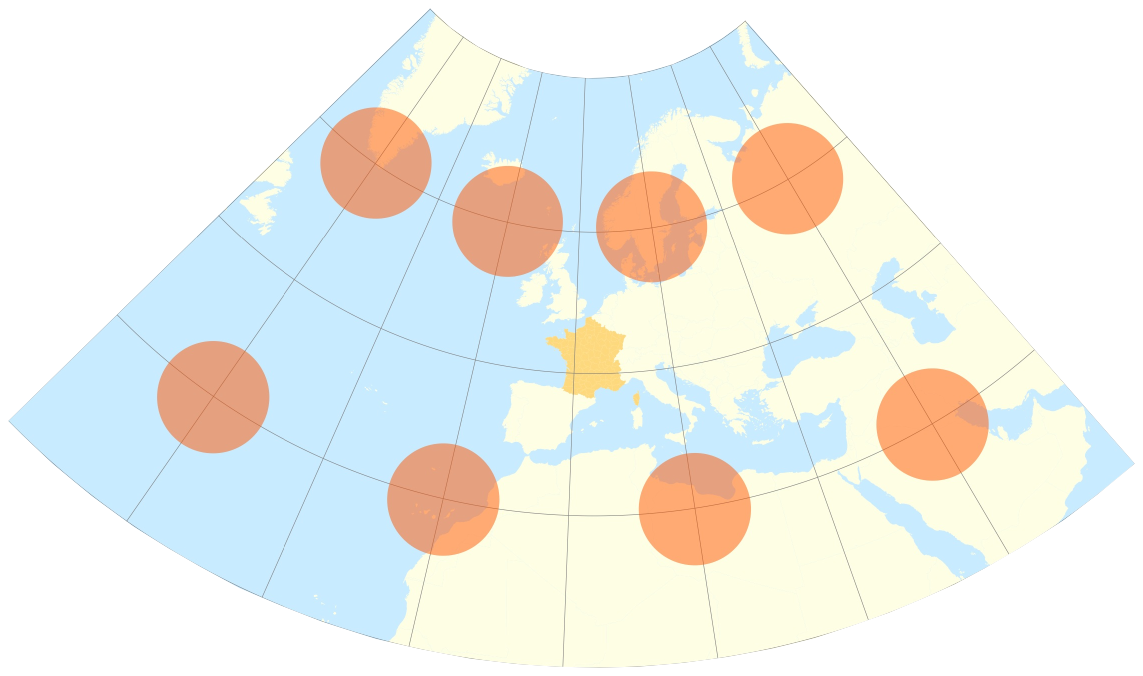
\includegraphics{figures/Lambert.png}
\end{frame}

\begin{frame}{Projection et calcul de distance}
\phantomsection\label{projection-et-calcul-de-distance-2}
\centering

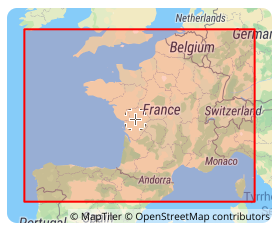
\includegraphics{figures/RGF93.png}
\end{frame}

\begin{frame}{Formats de fichiers fréquents}
\phantomsection\label{formats-de-fichiers-fruxe9quents}
Les données spatiales peuvent être stockées dans plusieurs formats.

Pour les données vectorielles :

\begin{itemize}
  \item \texttt{.shp} : shapefile, format très répandu ;
  \item \texttt{.gpkg} : GeoPackage, format plus moderne ;
  \item \texttt{.geojson} : format pratique pour le web.
\end{itemize}

Pour les données raster :

\begin{itemize}
  \item \texttt{.tif} ou \texttt{.tiff} : GeoTIFF ;
  \item \texttt{.nc} : NetCDF, souvent utilisé pour les données climatiques.
\end{itemize}

Bonne pratique : Pour les nouveaux projets, le format GeoPackage est
souvent plus pratique qu'un shapefile.
\end{frame}

\begin{frame}{L'objet sf dans R}
\phantomsection\label{lobjet-sf-dans-r}
Dans R, le package sf permet de manipuler des données vectorielles.

Un objet sf ressemble à un tableau de données classique.

La différence principale est qu'il contient une colonne spéciale :
\textbf{geometry}

Cette colonne contient les coordonnées ou les formes géographiques.
\end{frame}

\begin{frame}{L'objet sf}
\phantomsection\label{lobjet-sf}
\centering

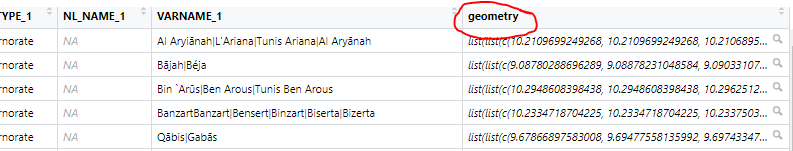
\includegraphics{figures/sf_object.png}
\end{frame}

\begin{frame}{Pourquoi sf est pratique ?}
\phantomsection\label{pourquoi-sf-est-pratique}
Comme un objet sf est proche d'un tableau classique, on peut souvent
utiliser les outils du tidyverse.

Par exemple, on peut :

\begin{itemize}
  \item sélectionner des variables avec \texttt{select()} ;
  \item filtrer des observations avec \texttt{filter()} ;
  \item créer des variables avec \texttt{mutate()} ;
  \item faire des jointures avec \texttt{left\_join()} ;
  \item agréger avec \texttt{group\_by()} et \texttt{summarise()}.
\end{itemize}
\end{frame}

\begin{frame}{Les opérations spatiales de base}
\phantomsection\label{les-opuxe9rations-spatiales-de-base}
Les données spatiales permettent de réaliser des opérations spécifiques.

Exemples :

\begin{itemize}
  \item calculer une distance entre deux objets ;
  \item savoir si un point se trouve dans un polygone ;
  \item créer une zone tampon autour d’un lieu ;
  \item agréger plusieurs polygones ;
  \item calculer une surface ;
  \item extraire une valeur raster dans une zone.
\end{itemize}
\end{frame}

\begin{frame}{Les erreurs classiques avec les objets spatiaux}
\phantomsection\label{les-erreurs-classiques-avec-les-objets-spatiaux}
Quelques erreurs sont très fréquentes.

\begin{itemize}
  \item Calculer une distance alors que les coordonnées sont en degrés.
  \item Joindre deux bases avec des codes géographiques incompatibles.
  \item Mélanger des objets avec des CRS différents.
  \item Oublier les valeurs manquantes après une jointure.
  \item Interpréter une carte sans regarder les classes de couleur.
  \item Confondre une carte descriptive avec une relation causale.
\end{itemize}
\end{frame}

\section{Lire et manipuler des données avec
sf}\label{lire-et-manipuler-des-donnuxe9es-avec-sf}

\begin{frame}[fragile]{Charger les packages utiles}
\phantomsection\label{charger-les-packages-utiles}
On commence par charger les packages nécessaires.

\begin{Shaded}
\begin{Highlighting}[]
\FunctionTok{library}\NormalTok{(tidyverse)}
\FunctionTok{library}\NormalTok{(sf)}
\end{Highlighting}
\end{Shaded}

Le package sf permet de lire, manipuler et sauvegarder des données
vectorielles.

Le package tidyverse permet d'utiliser les fonctions habituelles de
manipulation de données.

Bonne pratique : Toujours charger les packages au début du script pour
rendre le code plus lisible.
\end{frame}

\begin{frame}[fragile]{Importer une couche géographique}
\phantomsection\label{importer-une-couche-guxe9ographique}
On importe une couche spatiale avec la fonction st\_read().

\begin{Shaded}
\begin{Highlighting}[]
\NormalTok{world\_map }\OtherTok{\textless{}{-}} \FunctionTok{st\_read}\NormalTok{(}\StringTok{"data/raw/world{-}administrative{-}boundaries.shp"}\NormalTok{)}
\end{Highlighting}
\end{Shaded}

Cette commande crée un objet appelé world\_map.

L'objet contient :

\begin{itemize}
\item des variables attributaires ;
\item une colonne géographique ;
\item le système de coordonnées de la couche.
\end{itemize}

st\_read() est l'équivalent spatial de read\_csv().
\end{frame}

\begin{frame}[fragile]{Inspecter un objet sf}
\phantomsection\label{inspecter-un-objet-sf}
Un objet sf peut être inspecté comme une base de données classique.

\begin{Shaded}
\begin{Highlighting}[]
\FunctionTok{glimpse}\NormalTok{(world\_map)}

\FunctionTok{names}\NormalTok{(world\_map)}

\FunctionTok{head}\NormalTok{(world\_map)}
\end{Highlighting}
\end{Shaded}

On peut alors identifier :

\begin{itemize}
\item les variables disponibles ;
\item le nombre d’observations ;
\item les codes géographiques ;
\item la colonne de géométrie.
\end{itemize}

Avant toute carte, toujours regarder la structure de l'objet spatial.
\end{frame}

\begin{frame}[fragile]{Afficher rapidement la géométrie}
\phantomsection\label{afficher-rapidement-la-guxe9omuxe9trie}
On peut afficher uniquement la géométrie d'un objet sf.

\begin{Shaded}
\begin{Highlighting}[]
\FunctionTok{plot}\NormalTok{(}\FunctionTok{st\_geometry}\NormalTok{(world\_map))}
\end{Highlighting}
\end{Shaded}

Cette commande permet de vérifier rapidement :

\begin{itemize}
\item si la couche s’affiche correctement ;
\item si les formes géographiques semblent cohérentes ;
\item si l’étendue spatiale correspond à ce que l’on attend.
\end{itemize}

Bonne pratique : Un premier plot() permet souvent de repérer rapidement
un problème de géométrie ou de projection.
\end{frame}

\begin{frame}[fragile]{Vérifier le système de coordonnées}
\phantomsection\label{vuxe9rifier-le-systuxe8me-de-coordonnuxe9es}
Chaque couche spatiale possède un système de coordonnées.

On peut le vérifier avec :

\begin{Shaded}
\begin{Highlighting}[]
\FunctionTok{st\_crs}\NormalTok{(world\_map)}
\end{Highlighting}
\end{Shaded}

Cette commande indique notamment :

\begin{itemize}
\item le code EPSG ;
\item le nom du système de coordonnées ;
\item l’unité utilisée ;
\item la projection éventuelle.
\end{itemize}

Avant de calculer une distance ou une surface, toujours vérifier le CRS.
\end{frame}

\begin{frame}[fragile]{Sélectionner des variables}
\phantomsection\label{suxe9lectionner-des-variables}
Comme avec une base classique, on peut sélectionner certaines colonnes.

\begin{Shaded}
\begin{Highlighting}[]
\NormalTok{world\_small }\OtherTok{\textless{}{-}}\NormalTok{ world\_map }\SpecialCharTok{\%\textgreater{}\%}
  \FunctionTok{select}\NormalTok{(name, iso3, continent, geometry)}
\end{Highlighting}
\end{Shaded}

La colonne geometry contient les formes géographiques.

Même si elle n'est pas explicitement sélectionnée, sf conserve souvent
la géométrie active.
\end{frame}

\begin{frame}[fragile]{Filtrer des objets géographiques}
\phantomsection\label{filtrer-des-objets-guxe9ographiques}
On peut filtrer des pays, régions ou communes avec filter().

\begin{Shaded}
\begin{Highlighting}[]
\NormalTok{europe\_map }\OtherTok{\textless{}{-}}\NormalTok{ world\_map }\SpecialCharTok{\%\textgreater{}\%}
  \FunctionTok{filter}\NormalTok{(continent }\SpecialCharTok{==} \StringTok{"Europe"}\NormalTok{)}
\end{Highlighting}
\end{Shaded}

On peut ensuite afficher le résultat.

\begin{Shaded}
\begin{Highlighting}[]
\FunctionTok{plot}\NormalTok{(}\FunctionTok{st\_geometry}\NormalTok{(europe\_map))}
\end{Highlighting}
\end{Shaded}

Ex : Ici, on crée une nouvelle couche contenant uniquement les pays
européens.
\end{frame}

\begin{frame}[fragile]{Créer de nouvelles variables}
\phantomsection\label{cruxe9er-de-nouvelles-variables}
On peut créer de nouvelles variables comme dans une base classique.

\begin{Shaded}
\begin{Highlighting}[]
\NormalTok{world\_map }\OtherTok{\textless{}{-}}\NormalTok{ world\_map }\SpecialCharTok{\%\textgreater{}\%}
  \FunctionTok{mutate}\NormalTok{(}
    \AttributeTok{is\_europe =}\NormalTok{ continent }\SpecialCharTok{==} \StringTok{"Europe"}
\NormalTok{  )}
\end{Highlighting}
\end{Shaded}

Cette variable peut ensuite être utilisée :

\begin{itemize}
\item pour filtrer la base ;
\item pour colorer une carte ;
\item pour définir un groupe d’analyse.
\end{itemize}
\end{frame}

\begin{frame}[fragile]{Supprimer temporairement la géométrie}
\phantomsection\label{supprimer-temporairement-la-guxe9omuxe9trie}
Parfois, on souhaite travailler uniquement sur la table attributaire.

On peut retirer la géométrie avec :

\begin{Shaded}
\begin{Highlighting}[]
\NormalTok{world\_table }\OtherTok{\textless{}{-}}\NormalTok{ world\_map }\SpecialCharTok{\%\textgreater{}\%}
  \FunctionTok{st\_drop\_geometry}\NormalTok{()}
\end{Highlighting}
\end{Shaded}

Cela permet de produire des tableaux, des statistiques ou des
vérifications sans conserver les géométries.

Exemple :

\begin{Shaded}
\begin{Highlighting}[]
\NormalTok{world\_table }\SpecialCharTok{\%\textgreater{}\%}
  \FunctionTok{count}\NormalTok{(continent)}
\end{Highlighting}
\end{Shaded}

Bonne pratique : Utiliser st\_drop\_geometry() lorsque la géométrie
n'est pas nécessaire.
\end{frame}

\begin{frame}[fragile]{Transformer une projection}
\phantomsection\label{transformer-une-projection}
On peut changer le système de coordonnées avec st\_transform().

\begin{Shaded}
\begin{Highlighting}[]
\NormalTok{world\_map\_3857 }\OtherTok{\textless{}{-}}\NormalTok{ world\_map }\SpecialCharTok{\%\textgreater{}\%}
  \FunctionTok{st\_transform}\NormalTok{(}\DecValTok{3857}\NormalTok{)}
\end{Highlighting}
\end{Shaded}

Pour la France métropolitaine, on utilise souvent le Lambert-93 :

\begin{Shaded}
\begin{Highlighting}[]
\NormalTok{france\_map\_2154 }\OtherTok{\textless{}{-}}\NormalTok{ world\_map }\SpecialCharTok{\%\textgreater{}\%}
  \FunctionTok{filter}\NormalTok{(iso3 }\SpecialCharTok{==} \StringTok{"FRA"}\NormalTok{) }\SpecialCharTok{\%\textgreater{}\%}
  \FunctionTok{st\_transform}\NormalTok{(}\DecValTok{2154}\NormalTok{)}
\end{Highlighting}
\end{Shaded}

st\_transform() ne change pas la forme réelle des objets : il change
leur représentation dans un autre système de coordonnées.
\end{frame}

\begin{frame}[fragile]{Calculer une surface}
\phantomsection\label{calculer-une-surface}
Une fois la projection adaptée, on peut calculer des surfaces.

\begin{Shaded}
\begin{Highlighting}[]
\NormalTok{france\_map\_2154 }\OtherTok{\textless{}{-}}\NormalTok{ france\_map\_2154 }\SpecialCharTok{\%\textgreater{}\%}
  \FunctionTok{mutate}\NormalTok{(}
    \AttributeTok{area\_km2 =} \FunctionTok{as.numeric}\NormalTok{(}\FunctionTok{st\_area}\NormalTok{(geometry)) }\SpecialCharTok{/} \FloatTok{1e6}
\NormalTok{  )}
\end{Highlighting}
\end{Shaded}

La fonction st\_area() calcule la surface des géométries.

On divise par 1e6 pour passer de mètres carrés à kilomètres carrés.

\(\rightarrow\) Pour calculer une surface, utiliser une projection
adaptée et vérifier l'unité.
\end{frame}

\begin{frame}[fragile]{Calculer un centroïde}
\phantomsection\label{calculer-un-centrouxefde}
Un centroïde est un point qui résume la position d'un polygone.

\begin{Shaded}
\begin{Highlighting}[]
\NormalTok{world\_centroids }\OtherTok{\textless{}{-}}\NormalTok{ world\_map }\SpecialCharTok{\%\textgreater{}\%}
  \FunctionTok{st\_centroid}\NormalTok{()}
\end{Highlighting}
\end{Shaded}

Les centroïdes sont utiles pour :

\begin{itemize}
\item placer des labels ;
\item calculer des distances approximatives ;
\item représenter des points à partir de polygones ;
\item simplifier certaines opérations spatiales.
\end{itemize}

Attention : Le centroïde n'est pas toujours situé à l'intérieur du
polygone, notamment pour les formes complexes.
\end{frame}

\begin{frame}[fragile]{Agréger des polygones}
\phantomsection\label{agruxe9ger-des-polygones}
On peut agréger plusieurs polygones avec group\_by() et summarise().

\begin{Shaded}
\begin{Highlighting}[]
\NormalTok{continents\_map }\OtherTok{\textless{}{-}}\NormalTok{ world\_map }\SpecialCharTok{\%\textgreater{}\%}
  \FunctionTok{group\_by}\NormalTok{(continent) }\SpecialCharTok{\%\textgreater{}\%}
  \FunctionTok{summarise}\NormalTok{(}
    \AttributeTok{n\_countries =} \FunctionTok{n}\NormalTok{(),}
    \AttributeTok{.groups =} \StringTok{"drop"}
\NormalTok{  )}
\end{Highlighting}
\end{Shaded}

Cette opération permet de passer : pays \(\rightarrow\) continents

Avec sf, summarise() agrège aussi les géométries.
\end{frame}

\begin{frame}[fragile]{Créer une zone tampon}
\phantomsection\label{cruxe9er-une-zone-tampon}
Une zone tampon, ou \textit{buffer}, correspond à une zone autour d'un
objet spatial.

\begin{Shaded}
\begin{Highlighting}[]
\NormalTok{france\_buffer }\OtherTok{\textless{}{-}}\NormalTok{ france\_map\_2154 }\SpecialCharTok{\%\textgreater{}\%}
  \FunctionTok{st\_buffer}\NormalTok{(}\AttributeTok{dist =} \DecValTok{100000}\NormalTok{)}
\end{Highlighting}
\end{Shaded}

Ici, on crée une zone de 100 km autour de la France.

Les buffers sont utiles pour construire des variables d'exposition :

\begin{itemize}
\item être situé à moins de 10 km d’une route ;
\item être situé autour d’une école ;
\item être proche d’une frontière ;
\item être exposé à une infrastructure.
\end{itemize}

Attention : La distance du buffer dépend de l'unité du CRS utilisé.
\end{frame}

\begin{frame}[fragile]{Sauvegarder une couche spatiale}
\phantomsection\label{sauvegarder-une-couche-spatiale}
Après manipulation, on peut sauvegarder une nouvelle couche.

\begin{Shaded}
\begin{Highlighting}[]
\FunctionTok{st\_write}\NormalTok{(}
\NormalTok{  europe\_map,}
  \StringTok{"data/clean/europe\_map.gpkg"}\NormalTok{,}
  \AttributeTok{delete\_dsn =} \ConstantTok{TRUE}
\NormalTok{)}
\end{Highlighting}
\end{Shaded}

Le format .gpkg est pratique car il stocke les données et la géométrie
dans un seul fichier.

Bonne pratique : Sauvegarder les couches nettoyées dans un dossier
data/clean.
\end{frame}

\begin{frame}[fragile]{Chaîne simple de traitement}
\phantomsection\label{chauxeene-simple-de-traitement}
On peut regrouper plusieurs étapes dans une seule chaîne.

\begin{Shaded}
\begin{Highlighting}[]
\NormalTok{europe\_map }\OtherTok{\textless{}{-}}\NormalTok{ world\_map }\SpecialCharTok{\%\textgreater{}\%}
  \FunctionTok{filter}\NormalTok{(continent }\SpecialCharTok{==} \StringTok{"Europe"}\NormalTok{) }\SpecialCharTok{\%\textgreater{}\%}
  \FunctionTok{select}\NormalTok{(name, iso3, continent, geometry) }\SpecialCharTok{\%\textgreater{}\%}
  \FunctionTok{st\_transform}\NormalTok{(}\DecValTok{3035}\NormalTok{) }\SpecialCharTok{\%\textgreater{}\%}
  \FunctionTok{mutate}\NormalTok{(}
    \AttributeTok{area\_km2 =} \FunctionTok{as.numeric}\NormalTok{(}\FunctionTok{st\_area}\NormalTok{(geometry)) }\SpecialCharTok{/} \FloatTok{1e6}
\NormalTok{  )}
\end{Highlighting}
\end{Shaded}

Cette chaîne permet de :

\begin{itemize}
\item sélectionner l’Europe ;
\item garder quelques variables utiles ;
\item changer de projection ;
\item calculer une surface.
\end{itemize}
\end{frame}

\begin{frame}{À retenir}
\phantomsection\label{uxe0-retenir}
Le package sf permet de manipuler simplement les données vectorielles.

Les commandes principales à retenir sont :

\begin{itemize}
  \item \texttt{st\_read()} : importer une couche spatiale ;
  \item \texttt{st\_crs()} : vérifier le système de coordonnées ;
  \item \texttt{st\_transform()} : changer de projection ;
  \item \texttt{st\_geometry()} : accéder à la géométrie ;
  \item \texttt{st\_drop\_geometry()} : retirer la géométrie ;
  \item \texttt{st\_area()} : calculer une surface ;
  \item \texttt{st\_centroid()} : calculer des centroïdes ;
  \item \texttt{st\_buffer()} : créer une zone tampon ;
  \item \texttt{st\_write()} : sauvegarder une couche.
\end{itemize}
\end{frame}

\section{Produire une première
carte}\label{produire-une-premiuxe8re-carte}

\begin{frame}{Produire une première carte}
\phantomsection\label{produire-une-premiuxe8re-carte-1}
Dans ce bloc, nous allons produire nos premières cartes avec R.

Nous verrons trois approches complémentaires :

\begin{itemize}
  \item \texttt{plot()} : pour vérifier rapidement une couche spatiale ;
  \item \texttt{ggplot2} : pour produire une carte statique propre ;
  \item \texttt{tmap} et \texttt{mapview} : pour produire des cartes cartographiques ou interactives.
\end{itemize}
\end{frame}

\begin{frame}[fragile]{Une première carte avec plot()}
\phantomsection\label{une-premiuxe8re-carte-avec-plot}
La fonction plot() permet de visualiser rapidement un objet spatial.

\begin{Shaded}
\begin{Highlighting}[]
\FunctionTok{plot}\NormalTok{(}\FunctionTok{st\_geometry}\NormalTok{(world\_map))}
\end{Highlighting}
\end{Shaded}

On peut aussi représenter une variable attributaire.

\begin{Shaded}
\begin{Highlighting}[]
\FunctionTok{plot}\NormalTok{(world\_map[}\StringTok{"continent"}\NormalTok{])}
\end{Highlighting}
\end{Shaded}

plot() est très utile pour vérifier rapidement que les données
s'affichent correctement.
\end{frame}

\begin{frame}[fragile]{Une carte avec ggplot2}
\phantomsection\label{une-carte-avec-ggplot2}
On peut produire une carte avec ggplot2 en utilisant geom\_sf().

\begin{Shaded}
\begin{Highlighting}[]
\FunctionTok{ggplot}\NormalTok{(world\_map) }\SpecialCharTok{+}
  \FunctionTok{geom\_sf}\NormalTok{()}
\end{Highlighting}
\end{Shaded}

geom\_sf() reconnaît automatiquement la colonne de géométrie de l'objet
sf.
\end{frame}

\begin{frame}[fragile]{Colorer une carte par continent}
\phantomsection\label{colorer-une-carte-par-continent}
On peut utiliser une variable attributaire pour colorer les polygones.

\begin{Shaded}
\begin{Highlighting}[]
\NormalTok{map\_continent }\OtherTok{\textless{}{-}} \FunctionTok{ggplot}\NormalTok{(world\_map) }\SpecialCharTok{+}
  \FunctionTok{geom\_sf}\NormalTok{(}
    \FunctionTok{aes}\NormalTok{(}\AttributeTok{fill =}\NormalTok{ continent),}
    \AttributeTok{color =} \StringTok{"grey70"}\NormalTok{,}
    \AttributeTok{size =} \FloatTok{0.1}
\NormalTok{  ) }\SpecialCharTok{+}
  \FunctionTok{theme\_minimal}\NormalTok{() }\SpecialCharTok{+}
  \FunctionTok{labs}\NormalTok{(}
    \AttributeTok{title =} \StringTok{"Carte des continents"}\NormalTok{,}
    \AttributeTok{fill =} \StringTok{"Continent"}
\NormalTok{  )}

\NormalTok{map\_continent}
\end{Highlighting}
\end{Shaded}
\end{frame}

\begin{frame}[fragile]{Améliorer la lisibilité}
\phantomsection\label{amuxe9liorer-la-lisibilituxe9}
Une carte doit rester simple et lisible.

On peut supprimer les axes et simplifier l'apparence.

\begin{Shaded}
\begin{Highlighting}[]
\NormalTok{map\_continent }\OtherTok{\textless{}{-}} \FunctionTok{ggplot}\NormalTok{(world\_map) }\SpecialCharTok{+}
  \FunctionTok{geom\_sf}\NormalTok{(}
    \FunctionTok{aes}\NormalTok{(}\AttributeTok{fill =}\NormalTok{ continent),}
    \AttributeTok{color =} \StringTok{"grey70"}\NormalTok{,}
    \AttributeTok{size =} \FloatTok{0.1}
\NormalTok{  ) }\SpecialCharTok{+}
  \FunctionTok{theme\_minimal}\NormalTok{() }\SpecialCharTok{+}
  \FunctionTok{theme}\NormalTok{(}
    \AttributeTok{axis.title =} \FunctionTok{element\_blank}\NormalTok{(),}
    \AttributeTok{axis.text =} \FunctionTok{element\_blank}\NormalTok{(),}
    \AttributeTok{panel.grid =} \FunctionTok{element\_blank}\NormalTok{()}
\NormalTok{  ) }\SpecialCharTok{+}
  \FunctionTok{labs}\NormalTok{(}
    \AttributeTok{title =} \StringTok{"Carte des continents"}\NormalTok{,}
    \AttributeTok{fill =} \StringTok{"Continent"}\NormalTok{,}
    \AttributeTok{caption =} \StringTok{"Source : données administratives mondiales"}
\NormalTok{  )}

\NormalTok{map\_continent}
\end{Highlighting}
\end{Shaded}
\end{frame}

\begin{frame}{Carte qualitative ou quantitative ?}
\phantomsection\label{carte-qualitative-ou-quantitative}
Toutes les variables ne se cartographient pas de la même manière.

On distingue souvent :

\begin{itemize}
  \item les variables \textbf{qualitatives} : continent, région, type de zone ;
  \item les variables \textbf{quantitatives} : population, revenu, émissions, densité.
\end{itemize}

Exemples :

\begin{itemize}
  \item \texttt{continent} : variable qualitative ;
  \item \texttt{population} : variable quantitative ;
  \item \texttt{co2\_per\_capita} : variable quantitative.
\end{itemize}
\end{frame}

\begin{frame}[fragile]{Une carte quantitative}
\phantomsection\label{une-carte-quantitative}
Pour une variable quantitative, on utilise une échelle continue.

Exemple avec une variable de population si elle est disponible dans la
base :

\begin{Shaded}
\begin{Highlighting}[]
\FunctionTok{ggplot}\NormalTok{(world\_map) }\SpecialCharTok{+}
  \FunctionTok{geom\_sf}\NormalTok{(}
    \FunctionTok{aes}\NormalTok{(}\AttributeTok{fill =}\NormalTok{ population),}
    \AttributeTok{color =} \StringTok{"grey80"}\NormalTok{,}
    \AttributeTok{size =} \FloatTok{0.05}
\NormalTok{  ) }\SpecialCharTok{+}
  \FunctionTok{scale\_fill\_viridis\_c}\NormalTok{(}
    \AttributeTok{na.value =} \StringTok{"grey90"}
\NormalTok{  ) }\SpecialCharTok{+}
  \FunctionTok{theme\_minimal}\NormalTok{() }\SpecialCharTok{+}
  \FunctionTok{labs}\NormalTok{(}\AttributeTok{title =} \StringTok{"Population par pays"}\NormalTok{,}
    \AttributeTok{fill =} \StringTok{"Population"}\NormalTok{  )}
\end{Highlighting}
\end{Shaded}

Attention : Les variables très asymétriques peuvent être difficiles à
représenter avec une échelle continue.
\end{frame}

\begin{frame}[fragile]{Gérer les valeurs manquantes}
\phantomsection\label{guxe9rer-les-valeurs-manquantes}
Une carte peut contenir des pays ou zones sans données.

Il faut les rendre visibles.

\begin{Shaded}
\begin{Highlighting}[]
\FunctionTok{ggplot}\NormalTok{(world\_map) }\SpecialCharTok{+}
  \FunctionTok{geom\_sf}\NormalTok{(}
    \FunctionTok{aes}\NormalTok{(}\AttributeTok{fill =}\NormalTok{ population),}
    \AttributeTok{color =} \StringTok{"grey80"}\NormalTok{,}
    \AttributeTok{size =} \FloatTok{0.05}
\NormalTok{  ) }\SpecialCharTok{+}
  \FunctionTok{scale\_fill\_viridis\_c}\NormalTok{(}
    \AttributeTok{na.value =} \StringTok{"grey90"}
\NormalTok{  ) }\SpecialCharTok{+}
  \FunctionTok{theme\_minimal}\NormalTok{() }\SpecialCharTok{+}
  \FunctionTok{labs}\NormalTok{(}
    \AttributeTok{title =} \StringTok{"Population par pays"}\NormalTok{,}
    \AttributeTok{fill =} \StringTok{"Population"}\NormalTok{,}
    \AttributeTok{caption =} \StringTok{"Les zones en gris correspondent aux valeurs manquantes"}
\NormalTok{  )}
\end{Highlighting}
\end{Shaded}

Bonne pratique : Ne pas cacher les valeurs manquantes : elles font
partie de l'information.
\end{frame}

\begin{frame}[fragile]{Créer des classes}
\phantomsection\label{cruxe9er-des-classes}
Pour certaines cartes, une variable catégorisée est plus lisible qu'une
échelle continue.

\begin{Shaded}
\begin{Highlighting}[]
\NormalTok{world\_map }\OtherTok{\textless{}{-}}\NormalTok{ world\_map }\SpecialCharTok{\%\textgreater{}\%}
  \FunctionTok{mutate}\NormalTok{(}
    \AttributeTok{pop\_class =} \FunctionTok{cut}\NormalTok{(}
\NormalTok{      population,}
      \AttributeTok{breaks =} \FunctionTok{c}\NormalTok{(}\DecValTok{0}\NormalTok{, }\FloatTok{1e6}\NormalTok{, }\FloatTok{1e7}\NormalTok{, }\FloatTok{5e7}\NormalTok{, }\FloatTok{1e8}\NormalTok{, }\ConstantTok{Inf}\NormalTok{),}
      \AttributeTok{labels =} \FunctionTok{c}\NormalTok{(}
        \StringTok{"\textless{} 1 million"}\NormalTok{,}
        \StringTok{"1{-}10 millions"}\NormalTok{,}
        \StringTok{"10{-}50 millions"}\NormalTok{,}
        \StringTok{"50{-}100 millions"}\NormalTok{,}
        \StringTok{"\textgreater{} 100 millions"}
\NormalTok{      )}
\NormalTok{    )}
\NormalTok{  )}
\end{Highlighting}
\end{Shaded}

Attention : Le choix des classes influence fortement la lecture de la
carte.
\end{frame}

\begin{frame}[fragile]{Cartographier des classes}
\phantomsection\label{cartographier-des-classes}
Une fois la variable catégorielle créée, on peut la représenter.

\begin{Shaded}
\begin{Highlighting}[]
\FunctionTok{ggplot}\NormalTok{(world\_map) }\SpecialCharTok{+}
  \FunctionTok{geom\_sf}\NormalTok{(}
    \FunctionTok{aes}\NormalTok{(}\AttributeTok{fill =}\NormalTok{ pop\_class),}
    \AttributeTok{color =} \StringTok{"grey80"}\NormalTok{,}
    \AttributeTok{size =} \FloatTok{0.05}
\NormalTok{  ) }\SpecialCharTok{+}
  \FunctionTok{theme\_minimal}\NormalTok{() }\SpecialCharTok{+}
  \FunctionTok{labs}\NormalTok{(}
    \AttributeTok{title =} \StringTok{"Population par pays"}\NormalTok{,}
    \AttributeTok{fill =} \StringTok{"Classe de population"}
\NormalTok{  )}
\end{Highlighting}
\end{Shaded}

Les classes facilitent la lecture, mais elles simplifient l'information
initiale.
\end{frame}

\begin{frame}[fragile]{Une carte avec tmap}
\phantomsection\label{une-carte-avec-tmap}
Le package tmap est conçu spécifiquement pour faire des cartes.

\begin{Shaded}
\begin{Highlighting}[]
\FunctionTok{library}\NormalTok{(tmap)}

\FunctionTok{tm\_shape}\NormalTok{(world\_map) }\SpecialCharTok{+}
  \FunctionTok{tm\_polygons}\NormalTok{(}\StringTok{"continent"}\NormalTok{)}
\end{Highlighting}
\end{Shaded}

tmap est utile pour produire rapidement des cartes cartographiques
propres.

ggplot2 est très flexible ; tmap est souvent plus directement pensé pour
la cartographie.
\end{frame}

\begin{frame}[fragile]{Une carte interactive avec mapview}
\phantomsection\label{une-carte-interactive-avec-mapview}
Le package mapview permet de visualiser rapidement une couche sur une
carte interactive.

\begin{Shaded}
\begin{Highlighting}[]
\FunctionTok{library}\NormalTok{(mapview)}

\FunctionTok{mapview}\NormalTok{(world\_map)}
\end{Highlighting}
\end{Shaded}

On peut zoomer, se déplacer et explorer les objets spatiaux.

mapview est très utile pour explorer les données, mais moins adapté à
une figure finale d'article.
\end{frame}

\begin{frame}{Quel outil utiliser ?}
\phantomsection\label{quel-outil-utiliser}
Chaque outil a un usage différent.

\begin{itemize}
  \item \texttt{plot()} : vérifier rapidement les données ;
  \item \texttt{ggplot2} : produire des figures intégrées à un workflow tidyverse ;
  \item \texttt{tmap} : produire des cartes cartographiques rapidement ;
  \item \texttt{mapview} : explorer les données de manière interactive.
\end{itemize}

Pour un article ou un rapport, on privilégie souvent ggplot2 ou tmap.
Pour explorer les données, mapview est très pratique.
\end{frame}

\begin{frame}{Les choix qui comptent}
\phantomsection\label{les-choix-qui-comptent}
Une carte n'est jamais neutre.

Plusieurs choix influencent son interprétation :

\begin{itemize}
  \item la projection utilisée ;
  \item la variable représentée ;
  \item l’échelle de couleur ;
  \item le choix des classes ;
  \item la gestion des valeurs manquantes ;
  \item le niveau géographique retenu ;
  \item le titre et la légende.
\end{itemize}

Une carte doit être lue comme un résultat construit, pas comme une
simple image des données.
\end{frame}

\section{Joindre données statistiques et
carte}\label{joindre-donnuxe9es-statistiques-et-carte}

\begin{frame}{Joindre données statistiques et carte}
\phantomsection\label{joindre-donnuxe9es-statistiques-et-carte-1}
Une carte thématique combine généralement deux types de données.

\begin{itemize}
  \item une couche géographique : pays, régions, communes, districts ;
  \item une base statistique : population, revenu, émissions, indicateurs socio-économiques.
\end{itemize}

L'objectif est de joindre ces deux sources pour produire une carte
exploitable.
\end{frame}

\begin{frame}{Exemple de question}
\phantomsection\label{exemple-de-question}
Nous partons d'une question simple :

\begin{quote}
Comment les émissions de CO2 par habitant se répartissent-elles dans le monde ?
\end{quote}

Pour répondre à cette question, nous avons besoin :

\begin{itemize}
  \item d’une carte des pays du monde ;
  \item d’une base statistique sur les émissions de CO2 ;
  \item d’un identifiant commun pour faire la jointure ;
  \item d’une variable à cartographier.
\end{itemize}

Avant une jointure, il faut toujours identifier la clé commune entre les
deux bases.
\end{frame}

\begin{frame}[fragile]{Identifier la clé de jointure}
\phantomsection\label{identifier-la-cluxe9-de-jointure}
Pour joindre deux bases, il faut une variable commune.

Dans notre exemple :

\begin{itemize}
  \item la carte contient un code pays : \texttt{iso3} ;
  \item la base CO2 contient un code pays : \texttt{iso\_code}.
\end{itemize}

On va donc joindre les deux bases avec :

\begin{Shaded}
\begin{Highlighting}[]
\NormalTok{world\_co2 }\OtherTok{\textless{}{-}}\NormalTok{ world\_map }\SpecialCharTok{\%\textgreater{}\%}
  \FunctionTok{left\_join}\NormalTok{(}
\NormalTok{    co2\_2019,}
    \AttributeTok{by =} \FunctionTok{c}\NormalTok{(}\StringTok{"iso3"} \OtherTok{=} \StringTok{"iso\_code"}\NormalTok{)}
\NormalTok{  )}
\end{Highlighting}
\end{Shaded}

Attention : Une grande partie des erreurs de carte vient de jointures
mal faites.
\end{frame}

\begin{frame}[fragile]{Importer la base statistique}
\phantomsection\label{importer-la-base-statistique}
On commence par importer la base CO2.

\begin{Shaded}
\begin{Highlighting}[]
\NormalTok{co2\_raw }\OtherTok{\textless{}{-}} \FunctionTok{read\_csv}\NormalTok{(}\StringTok{"data/raw/owid{-}co2{-}data.csv"}\NormalTok{)}
\end{Highlighting}
\end{Shaded}

On garde ensuite l'année 2019 et quelques variables utiles.

\begin{Shaded}
\begin{Highlighting}[]
\NormalTok{co2\_2019 }\OtherTok{\textless{}{-}}\NormalTok{ co2\_raw }\SpecialCharTok{\%\textgreater{}\%}
  \FunctionTok{filter}\NormalTok{(year }\SpecialCharTok{==} \DecValTok{2019}\NormalTok{) }\SpecialCharTok{\%\textgreater{}\%}
  \FunctionTok{select}\NormalTok{(}
\NormalTok{    iso\_code, country, year,}
\NormalTok{    co2\_per\_capita, population, gdp}
\NormalTok{  )}
\end{Highlighting}
\end{Shaded}

Bonne pratique : Avant de joindre, créer une base statistique simple
avec uniquement les variables utiles.
\end{frame}

\begin{frame}[fragile]{Vérifier la base à joindre}
\phantomsection\label{vuxe9rifier-la-base-uxe0-joindre}
Avant la jointure, on inspecte rapidement la base statistique.

\begin{Shaded}
\begin{Highlighting}[]
\FunctionTok{glimpse}\NormalTok{(co2\_2019)}

\NormalTok{co2\_2019 }\SpecialCharTok{\%\textgreater{}\%}
  \FunctionTok{summarise}\NormalTok{(}
    \AttributeTok{n\_obs =} \FunctionTok{n}\NormalTok{(),}
    \AttributeTok{n\_countries =} \FunctionTok{n\_distinct}\NormalTok{(iso\_code),}
    \AttributeTok{missing\_co2\_pc =} \FunctionTok{sum}\NormalTok{(}\FunctionTok{is.na}\NormalTok{(co2\_per\_capita))}
\NormalTok{  )}
\end{Highlighting}
\end{Shaded}

On peut aussi vérifier les codes pays manquants.

\begin{Shaded}
\begin{Highlighting}[]
\NormalTok{co2\_2019 }\SpecialCharTok{\%\textgreater{}\%}
  \FunctionTok{filter}\NormalTok{(}\FunctionTok{is.na}\NormalTok{(iso\_code)) }\SpecialCharTok{\%\textgreater{}\%}
  \FunctionTok{select}\NormalTok{(country)}
\end{Highlighting}
\end{Shaded}

Toujours vérifier la base statistique avant de la joindre à une carte.
\end{frame}

\begin{frame}[fragile]{Réaliser la jointure}
\phantomsection\label{ruxe9aliser-la-jointure}
On joint la base statistique à la carte avec left\_join().

\begin{Shaded}
\begin{Highlighting}[]
\NormalTok{world\_co2 }\OtherTok{\textless{}{-}}\NormalTok{ world\_map }\SpecialCharTok{\%\textgreater{}\%}
  \FunctionTok{left\_join}\NormalTok{(}
\NormalTok{    co2\_2019,}
    \AttributeTok{by =} \FunctionTok{c}\NormalTok{(}\StringTok{"iso3"} \OtherTok{=} \StringTok{"iso\_code"}\NormalTok{)}
\NormalTok{  )}
\end{Highlighting}
\end{Shaded}

Ici, on garde toutes les géométries de la carte et on ajoute les
variables CO2 lorsqu'une correspondance existe.
\end{frame}

\begin{frame}[fragile]{Vérifier le résultat de la jointure}
\phantomsection\label{vuxe9rifier-le-ruxe9sultat-de-la-jointure}
Après une jointure, il faut toujours vérifier ce qui a été apparié ou
non.

\begin{Shaded}
\begin{Highlighting}[]
\NormalTok{world\_co2 }\SpecialCharTok{\%\textgreater{}\%}
  \FunctionTok{summarise}\NormalTok{(}
    \AttributeTok{n\_polygons =} \FunctionTok{n}\NormalTok{(),}
    \AttributeTok{matched\_co2 =} \FunctionTok{sum}\NormalTok{(}\SpecialCharTok{!}\FunctionTok{is.na}\NormalTok{(co2\_per\_capita)),}
    \AttributeTok{missing\_co2 =} \FunctionTok{sum}\NormalTok{(}\FunctionTok{is.na}\NormalTok{(co2\_per\_capita))}
\NormalTok{  )}
\end{Highlighting}
\end{Shaded}

On peut aussi afficher les pays sans données CO2.

\begin{Shaded}
\begin{Highlighting}[]
\NormalTok{world\_co2 }\SpecialCharTok{\%\textgreater{}\%}
  \FunctionTok{filter}\NormalTok{(}\FunctionTok{is.na}\NormalTok{(co2\_per\_capita)) }\SpecialCharTok{\%\textgreater{}\%}
  \FunctionTok{st\_drop\_geometry}\NormalTok{() }\SpecialCharTok{\%\textgreater{}\%}
  \FunctionTok{select}\NormalTok{(name, iso3)}
\end{Highlighting}
\end{Shaded}

Bonne pratique : Une jointure doit toujours être contrôlée : certaines
unités peuvent ne pas être appariées.
\end{frame}

\begin{frame}{Comprendre les non-appariements}
\phantomsection\label{comprendre-les-non-appariements}
Les non-appariements peuvent venir de plusieurs sources.

\begin{itemize}
  \item codes pays différents ;
  \item territoires présents dans la carte mais absents de la base statistique ;
  \item agrégats présents dans la base statistique mais absents de la carte ;
  \item changements de frontières ou de noms ;
  \item valeurs manquantes pour certaines années.
\end{itemize}

Exemples fréquents :

\begin{itemize}
  \item Kosovo ;
  \item territoires ultramarins ;
  \item petits États insulaires ;
  \item régions ou agrégats comme \textit{World}, \textit{Europe}, \textit{Asia}.
\end{itemize}

Un pays non apparié n'est pas forcément une erreur, mais il doit être
identifié.
\end{frame}

\begin{frame}[fragile]{Première carte des émissions de CO2}
\phantomsection\label{premiuxe8re-carte-des-uxe9missions-de-co2}
Une fois la jointure réalisée, on peut cartographier la variable.

\begin{Shaded}
\begin{Highlighting}[]
\FunctionTok{ggplot}\NormalTok{(world\_co2) }\SpecialCharTok{+}
  \FunctionTok{geom\_sf}\NormalTok{(}
    \FunctionTok{aes}\NormalTok{(}\AttributeTok{fill =}\NormalTok{ co2\_per\_capita),}
    \AttributeTok{color =} \StringTok{"grey80"}\NormalTok{,}
    \AttributeTok{size =} \FloatTok{0.05}
\NormalTok{  ) }\SpecialCharTok{+}
  \FunctionTok{scale\_fill\_viridis\_c}\NormalTok{(}
    \AttributeTok{na.value =} \StringTok{"grey90"}
\NormalTok{  ) }\SpecialCharTok{+}
  \FunctionTok{theme\_minimal}\NormalTok{() }\SpecialCharTok{+}
  \FunctionTok{labs}\NormalTok{(}
    \AttributeTok{title =} \StringTok{"Émissions de CO2 par habitant en 2019"}\NormalTok{,}
    \AttributeTok{fill =} \StringTok{"CO2 par habitant"}\NormalTok{,}
    \AttributeTok{caption =} \StringTok{"Source : Our World in Data"}
\NormalTok{  )}
\end{Highlighting}
\end{Shaded}

Les pays en gris correspondent aux pays sans valeur disponible ou non
appariés.
\end{frame}

\begin{frame}[fragile]{Rendre la carte plus lisible}
\phantomsection\label{rendre-la-carte-plus-lisible}
Pour une carte thématique, on peut simplifier l'apparence.

\begin{Shaded}
\begin{Highlighting}[]
\NormalTok{map\_co2\_2019 }\OtherTok{\textless{}{-}} \FunctionTok{ggplot}\NormalTok{(world\_co2) }\SpecialCharTok{+}
  \FunctionTok{geom\_sf}\NormalTok{(}
    \FunctionTok{aes}\NormalTok{(}\AttributeTok{fill =}\NormalTok{ co2\_per\_capita),}
    \AttributeTok{color =} \StringTok{"grey80"}\NormalTok{,}
    \AttributeTok{size =} \FloatTok{0.05}
\NormalTok{  ) }\SpecialCharTok{+}
  \FunctionTok{scale\_fill\_viridis\_c}\NormalTok{(}
    \AttributeTok{na.value =} \StringTok{"grey90"}
\NormalTok{  ) }\SpecialCharTok{+}
  \FunctionTok{theme\_minimal}\NormalTok{() }\SpecialCharTok{+}
  \FunctionTok{theme}\NormalTok{(}
    \AttributeTok{axis.title =} \FunctionTok{element\_blank}\NormalTok{(),}
    \AttributeTok{axis.text =} \FunctionTok{element\_blank}\NormalTok{(),}
    \AttributeTok{panel.grid =} \FunctionTok{element\_blank}\NormalTok{()}
\NormalTok{  ) }\SpecialCharTok{+}
  \FunctionTok{labs}\NormalTok{(}
    \AttributeTok{title =} \StringTok{"Émissions de CO2 par habitant en 2019"}\NormalTok{,}
    \AttributeTok{fill =} \StringTok{"CO2 par habitant"}\NormalTok{,}
    \AttributeTok{caption =} \StringTok{"Source : Our World in Data"}
\NormalTok{  )}

\NormalTok{map\_co2\_2019}
\end{Highlighting}
\end{Shaded}

Bonne pratique : Une carte finale doit avoir un titre clair, une légende
lisible et une source.
\end{frame}

\begin{frame}[fragile]{Créer des classes de valeurs}
\phantomsection\label{cruxe9er-des-classes-de-valeurs}
Pour certaines variables très asymétriques, une carte en classes peut
être plus lisible.

\begin{Shaded}
\begin{Highlighting}[]
\NormalTok{world\_co2 }\OtherTok{\textless{}{-}}\NormalTok{ world\_co2 }\SpecialCharTok{\%\textgreater{}\%}
  \FunctionTok{mutate}\NormalTok{(}
    \AttributeTok{co2\_class =} \FunctionTok{cut}\NormalTok{(}
\NormalTok{      co2\_per\_capita,}
      \AttributeTok{breaks =} \FunctionTok{c}\NormalTok{(}\DecValTok{0}\NormalTok{, }\DecValTok{1}\NormalTok{, }\DecValTok{3}\NormalTok{, }\DecValTok{5}\NormalTok{, }\DecValTok{10}\NormalTok{, }\DecValTok{20}\NormalTok{, }\ConstantTok{Inf}\NormalTok{),}
      \AttributeTok{labels =} \FunctionTok{c}\NormalTok{(}
        \StringTok{"\textless{} 1"}\NormalTok{,}
        \StringTok{"1{-}3"}\NormalTok{,}
        \StringTok{"3{-}5"}\NormalTok{,}
        \StringTok{"5{-}10"}\NormalTok{,}
        \StringTok{"10{-}20"}\NormalTok{,}
        \StringTok{"\textgreater{} 20"}
\NormalTok{      )}
\NormalTok{    )}
\NormalTok{  )}
\end{Highlighting}
\end{Shaded}

Attention : Le choix des seuils influence fortement la lecture de la
carte.
\end{frame}

\begin{frame}[fragile]{Cartographier les classes}
\phantomsection\label{cartographier-les-classes}
On peut ensuite représenter la variable catégorisée.

\begin{Shaded}
\begin{Highlighting}[]
\FunctionTok{ggplot}\NormalTok{(world\_co2) }\SpecialCharTok{+}
  \FunctionTok{geom\_sf}\NormalTok{(}
    \FunctionTok{aes}\NormalTok{(}\AttributeTok{fill =}\NormalTok{ co2\_class),}
    \AttributeTok{color =} \StringTok{"grey80"}\NormalTok{,}
    \AttributeTok{size =} \FloatTok{0.05}
\NormalTok{  ) }\SpecialCharTok{+}
  \FunctionTok{theme\_minimal}\NormalTok{() }\SpecialCharTok{+}
  \FunctionTok{theme}\NormalTok{(}
    \AttributeTok{axis.title =} \FunctionTok{element\_blank}\NormalTok{(),}
    \AttributeTok{axis.text =} \FunctionTok{element\_blank}\NormalTok{(),}
    \AttributeTok{panel.grid =} \FunctionTok{element\_blank}\NormalTok{()}
\NormalTok{  ) }\SpecialCharTok{+}
  \FunctionTok{labs}\NormalTok{(}
    \AttributeTok{title =} \StringTok{"Émissions de CO2 par habitant en 2019"}\NormalTok{,}
    \AttributeTok{fill =} \StringTok{"Tonnes par habitant"}\NormalTok{,}
    \AttributeTok{caption =} \StringTok{"Source : Our World in Data"}
\NormalTok{  )}
\end{Highlighting}
\end{Shaded}

Les classes facilitent la lecture, mais elles simplifient une variable
continue.
\end{frame}

\begin{frame}[fragile]{Comparer deux variables cartographiées}
\phantomsection\label{comparer-deux-variables-cartographiuxe9es}
Une fois la jointure faite, on peut cartographier différentes variables.

Par exemple, la population :

\begin{Shaded}
\begin{Highlighting}[]
\FunctionTok{ggplot}\NormalTok{(world\_co2) }\SpecialCharTok{+}
  \FunctionTok{geom\_sf}\NormalTok{(}
    \FunctionTok{aes}\NormalTok{(}\AttributeTok{fill =}\NormalTok{ population),}
    \AttributeTok{color =} \StringTok{"grey80"}\NormalTok{,}
    \AttributeTok{size =} \FloatTok{0.05}
\NormalTok{  ) }\SpecialCharTok{+}
  \FunctionTok{scale\_fill\_viridis\_c}\NormalTok{(}
    \AttributeTok{trans =} \StringTok{"log10"}\NormalTok{,}
    \AttributeTok{na.value =} \StringTok{"grey90"}
\NormalTok{  ) }\SpecialCharTok{+}
  \FunctionTok{theme\_minimal}\NormalTok{() }\SpecialCharTok{+}
  \FunctionTok{labs}\NormalTok{(}
    \AttributeTok{title =} \StringTok{"Population par pays en 2019"}\NormalTok{,}
    \AttributeTok{fill =} \StringTok{"Population"}\NormalTok{,}
    \AttributeTok{caption =} \StringTok{"Source : Our World in Data"}
\NormalTok{  )}
\end{Highlighting}
\end{Shaded}
\end{frame}

\begin{frame}{Attention aux échelles}
\phantomsection\label{attention-aux-uxe9chelles}
Les cartes peuvent donner des impressions différentes selon la variable
représentée.

Exemples :

\begin{itemize}
  \item émissions totales de CO2 ;
  \item émissions de CO2 par habitant ;
  \item PIB total ;
  \item PIB par habitant ;
  \item population ;
  \item densité de population.
\end{itemize}

Ces variables ne répondent pas aux mêmes questions.
\end{frame}

\begin{frame}{Carte et interprétation}
\phantomsection\label{carte-et-interpruxe9tation}
Une carte des émissions de CO2 par habitant permet de visualiser des
différences spatiales.

Mais elle ne permet pas directement d'expliquer ces différences.

Pour interpréter la carte, il faut tenir compte :

\begin{itemize}
  \item du niveau de développement ;
  \item de la structure productive ;
  \item de la géographie ;
  \item des ressources énergétiques ;
  \item de la population ;
  \item des choix de mesure.
\end{itemize}

Une carte décrit une distribution spatiale ; elle ne suffit pas à
identifier une relation causale.
\end{frame}

\begin{frame}[fragile]{Sauvegarder la carte}
\phantomsection\label{sauvegarder-la-carte}
On peut sauvegarder une carte avec ggsave().

\begin{Shaded}
\begin{Highlighting}[]
\FunctionTok{ggsave}\NormalTok{(}
  \AttributeTok{filename =} \StringTok{"outputs/figures/map\_co2\_2019.png"}\NormalTok{,}
  \AttributeTok{plot =}\NormalTok{ map\_co2\_2019,}
  \AttributeTok{width =} \DecValTok{10}\NormalTok{,}
  \AttributeTok{height =} \DecValTok{6}\NormalTok{,}
  \AttributeTok{dpi =} \DecValTok{300}
\NormalTok{)}
\end{Highlighting}
\end{Shaded}

Cela permet de réutiliser la carte dans :

\begin{itemize}
\item un article ;
\item un rapport ;
\item une présentation ;
\item un document RMarkdown.
\end{itemize}

Bonne pratique : Sauvegarder les figures produites dans un dossier
outputs/figures.
\end{frame}

\section{Points, distances et
intersections}\label{points-distances-et-intersections}

\begin{frame}{Points, distances et intersections}
\phantomsection\label{points-distances-et-intersections-1}
Les données spatiales ne servent pas seulement à produire des cartes.

Elles permettent aussi de construire des variables utiles pour l'analyse
empirique.

Dans ce bloc, nous allons voir comment :

\begin{itemize}
  \item manipuler des données ponctuelles ;
  \item convertir une table avec coordonnées en objet spatial ;
  \item projeter des points sur une carte ;
  \item calculer des distances ;
  \item compter des points dans des polygones ;
  \item identifier des intersections spatiales.
\end{itemize}
\end{frame}

\begin{frame}{Pourquoi travailler avec des points ?}
\phantomsection\label{pourquoi-travailler-avec-des-points}
De nombreuses données utilisées en économie appliquée sont localisées
par des coordonnées.

Exemples :

\begin{itemize}
  \item écoles ;
  \item ménages ;
  \item entreprises ;
  \item hôpitaux ;
  \item antennes téléphoniques ;
  \item centrales électriques ;
  \item conflits ou manifestations ;
  \item infrastructures publiques.
\end{itemize}

Ces observations peuvent être représentées comme des points.

Dès qu'une observation a une latitude et une longitude, elle peut
devenir une donnée spatiale.
\end{frame}

\begin{frame}{Exemple de question empirique}
\phantomsection\label{exemple-de-question-empirique}
Supposons que l'on dispose de la localisation de centrales électriques.

On peut se poser plusieurs questions :

\begin{itemize}
  \item Dans quels pays ces centrales sont-elles situées ?
  \item Combien de centrales se trouvent dans chaque pays ?
  \item Quelle est la distance entre chaque pays et la centrale la plus proche ?
  \item Quels territoires sont situés à moins de 50 km d’une centrale ?
  \item Les zones proches d’une infrastructure ont-elles des trajectoires économiques différentes ?
\end{itemize}

Ex : Transformer des coordonnées géographiques en variables d'exposition
à une infrastructure.
\end{frame}

\begin{frame}[fragile]{Charger une base de points}
\phantomsection\label{charger-une-base-de-points}
On peut lire une couche de points comme n'importe quelle couche
spatiale.

\begin{Shaded}
\begin{Highlighting}[]
\NormalTok{power\_plants }\OtherTok{\textless{}{-}} \FunctionTok{st\_read}\NormalTok{(}\StringTok{"data/raw/Global\_Power\_Plants/Power\_Plants.shp"}\NormalTok{)}
\end{Highlighting}
\end{Shaded}

On inspecte ensuite l'objet.

\begin{Shaded}
\begin{Highlighting}[]
\FunctionTok{glimpse}\NormalTok{(power\_plants)}

\FunctionTok{st\_crs}\NormalTok{(power\_plants)}

\FunctionTok{plot}\NormalTok{(}\FunctionTok{st\_geometry}\NormalTok{(power\_plants))}
\end{Highlighting}
\end{Shaded}

Comme pour les polygones, on vérifie toujours la structure, la géométrie
et le CRS.
\end{frame}

\begin{frame}[fragile]{Créer des points à partir de coordonnées}
\phantomsection\label{cruxe9er-des-points-uxe0-partir-de-coordonnuxe9es}
Parfois, les données ne sont pas encore spatiales.

Elles peuvent simplement contenir deux colonnes :

\[
\text{longitude}, \text{latitude}
\]

On peut les convertir en objet sf avec st\_as\_sf().

\begin{Shaded}
\begin{Highlighting}[]
\NormalTok{power\_plants\_sf }\OtherTok{\textless{}{-}}\NormalTok{ power\_plants\_df }\SpecialCharTok{\%\textgreater{}\%}
  \FunctionTok{st\_as\_sf}\NormalTok{(}
    \AttributeTok{coords =} \FunctionTok{c}\NormalTok{(}\StringTok{"longitude"}\NormalTok{, }\StringTok{"latitude"}\NormalTok{),}
    \AttributeTok{crs =} \DecValTok{4326}
\NormalTok{  )}
\end{Highlighting}
\end{Shaded}

Attention : Il faut indiquer le bon CRS : les coordonnées
longitude-latitude sont généralement en EPSG:4326.
\end{frame}

\begin{frame}[fragile]{Afficher des points sur une carte}
\phantomsection\label{afficher-des-points-sur-une-carte}
On peut superposer les points à une carte de polygones.

\begin{Shaded}
\begin{Highlighting}[]
\FunctionTok{ggplot}\NormalTok{() }\SpecialCharTok{+}
  \FunctionTok{geom\_sf}\NormalTok{(}\AttributeTok{data =}\NormalTok{ world\_map, }\AttributeTok{fill =} \StringTok{"grey95"}\NormalTok{, }\AttributeTok{color =} \StringTok{"grey80"}\NormalTok{) }\SpecialCharTok{+}
  \FunctionTok{geom\_sf}\NormalTok{(}\AttributeTok{data =}\NormalTok{ power\_plants, }\AttributeTok{size =} \FloatTok{0.5}\NormalTok{, }\AttributeTok{alpha =} \FloatTok{0.6}\NormalTok{) }\SpecialCharTok{+}
  \FunctionTok{theme\_minimal}\NormalTok{() }\SpecialCharTok{+}
  \FunctionTok{labs}\NormalTok{(}
    \AttributeTok{title =} \StringTok{"Localisation des centrales électriques"}
\NormalTok{  )}
\end{Highlighting}
\end{Shaded}

Les polygones donnent le contexte géographique ; les points représentent
les unités localisées.
\end{frame}

\begin{frame}[fragile]{Filtrer un type de points}
\phantomsection\label{filtrer-un-type-de-points}
Si la base contient plusieurs types d'infrastructures, on peut filtrer
les observations.

\begin{Shaded}
\begin{Highlighting}[]
\NormalTok{nuclear\_plants }\OtherTok{\textless{}{-}}\NormalTok{ power\_plants }\SpecialCharTok{\%\textgreater{}\%}
  \FunctionTok{filter}\NormalTok{(fuel1 }\SpecialCharTok{==} \StringTok{"Nuclear"}\NormalTok{)}
\end{Highlighting}
\end{Shaded}

Puis afficher uniquement ces points.

\begin{Shaded}
\begin{Highlighting}[]
\FunctionTok{ggplot}\NormalTok{() }\SpecialCharTok{+}
  \FunctionTok{geom\_sf}\NormalTok{(}\AttributeTok{data =}\NormalTok{ world\_map, }\AttributeTok{fill =} \StringTok{"grey95"}\NormalTok{, }\AttributeTok{color =} \StringTok{"grey80"}\NormalTok{) }\SpecialCharTok{+}
  \FunctionTok{geom\_sf}\NormalTok{(}\AttributeTok{data =}\NormalTok{ nuclear\_plants, }\AttributeTok{size =} \FloatTok{0.8}\NormalTok{, }\AttributeTok{alpha =} \FloatTok{0.7}\NormalTok{) }\SpecialCharTok{+}
  \FunctionTok{theme\_minimal}\NormalTok{() }\SpecialCharTok{+}
  \FunctionTok{labs}\NormalTok{(}
    \AttributeTok{title =} \StringTok{"Centrales nucléaires"}
\NormalTok{  )}
\end{Highlighting}
\end{Shaded}

Ex : On peut isoler un type d'infrastructure pour construire une
variable d'exposition spécifique.
\end{frame}

\begin{frame}[fragile]{Harmoniser les projections}
\phantomsection\label{harmoniser-les-projections}
Avant certaines opérations spatiales, les objets doivent avoir le même
CRS.

\begin{Shaded}
\begin{Highlighting}[]
\FunctionTok{st\_crs}\NormalTok{(world\_map)}
\FunctionTok{st\_crs}\NormalTok{(power\_plants)}
\end{Highlighting}
\end{Shaded}

Si nécessaire, on transforme la projection.

\begin{Shaded}
\begin{Highlighting}[]
\NormalTok{power\_plants }\OtherTok{\textless{}{-}} \FunctionTok{st\_transform}\NormalTok{(power\_plants, }\FunctionTok{st\_crs}\NormalTok{(world\_map))}
\end{Highlighting}
\end{Shaded}

Avant une intersection, une distance ou une jointure spatiale, vérifier
que les CRS sont compatibles.
\end{frame}

\begin{frame}[fragile]{Sélectionner une zone d'étude}
\phantomsection\label{suxe9lectionner-une-zone-duxe9tude}
On peut restreindre l'analyse à une zone géographique.

\begin{Shaded}
\begin{Highlighting}[]
\NormalTok{europe\_map }\OtherTok{\textless{}{-}}\NormalTok{ world\_map }\SpecialCharTok{\%\textgreater{}\%}
  \FunctionTok{filter}\NormalTok{(continent }\SpecialCharTok{==} \StringTok{"Europe"}\NormalTok{)}
\end{Highlighting}
\end{Shaded}

On peut ensuite garder les points situés dans cette zone.

\begin{Shaded}
\begin{Highlighting}[]
\NormalTok{power\_plants\_europe }\OtherTok{\textless{}{-}}\NormalTok{ power\_plants }\SpecialCharTok{\%\textgreater{}\%}
  \FunctionTok{st\_filter}\NormalTok{(europe\_map)}
\end{Highlighting}
\end{Shaded}

st\_filter() permet de garder les objets qui intersectent une couche
spatiale.
\end{frame}

\begin{frame}[fragile]{Points dans polygones}
\phantomsection\label{points-dans-polygones}
Une opération classique consiste à identifier dans quel polygone se
trouve chaque point.

\begin{Shaded}
\begin{Highlighting}[]
\NormalTok{plants\_with\_country }\OtherTok{\textless{}{-}}\NormalTok{ power\_plants }\SpecialCharTok{\%\textgreater{}\%}
  \FunctionTok{st\_join}\NormalTok{(world\_map)}
\end{Highlighting}
\end{Shaded}

Cette opération ajoute aux points les informations du polygone dans
lequel ils se trouvent.

Exemple :

\begin{itemize}
\item une centrale reçoit le code du pays où elle est localisée ;
\item une école reçoit le nom de la commune ;
\item un ménage reçoit l’identifiant du district.
\end{itemize}
\end{frame}

\begin{frame}[fragile]{Compter des points dans des polygones}
\phantomsection\label{compter-des-points-dans-des-polygones}
On peut compter le nombre de points dans chaque pays ou région.

\begin{Shaded}
\begin{Highlighting}[]
\NormalTok{points\_in\_country }\OtherTok{\textless{}{-}} \FunctionTok{st\_intersects}\NormalTok{(world\_map, power\_plants)}

\NormalTok{world\_map}\SpecialCharTok{$}\NormalTok{n\_power\_plants }\OtherTok{\textless{}{-}} \FunctionTok{lengths}\NormalTok{(points\_in\_country)}
\end{Highlighting}
\end{Shaded}

La variable n\_power\_plants indique le nombre de centrales dans chaque
pays.

Ex : Construire le nombre d'infrastructures disponibles dans une unité
administrative.
\end{frame}

\begin{frame}[fragile]{Cartographier un comptage}
\phantomsection\label{cartographier-un-comptage}
Une fois le nombre de points calculé, on peut produire une carte.

\begin{Shaded}
\begin{Highlighting}[]
\FunctionTok{ggplot}\NormalTok{(world\_map) }\SpecialCharTok{+}
  \FunctionTok{geom\_sf}\NormalTok{(}
    \FunctionTok{aes}\NormalTok{(}\AttributeTok{fill =}\NormalTok{ n\_power\_plants),}
    \AttributeTok{color =} \StringTok{"grey80"}\NormalTok{,}
    \AttributeTok{size =} \FloatTok{0.05}
\NormalTok{  ) }\SpecialCharTok{+}
  \FunctionTok{scale\_fill\_viridis\_c}\NormalTok{(}
    \AttributeTok{na.value =} \StringTok{"grey90"}
\NormalTok{  ) }\SpecialCharTok{+}
  \FunctionTok{theme\_minimal}\NormalTok{() }\SpecialCharTok{+}
  \FunctionTok{labs}\NormalTok{(}
    \AttributeTok{title =} \StringTok{"Nombre de centrales électriques par pays"}\NormalTok{,}
    \AttributeTok{fill =} \StringTok{"Nombre"}
\NormalTok{  )}
\end{Highlighting}
\end{Shaded}

Attention : Un nombre total dépend souvent de la taille du pays : une
densité peut parfois être plus informative.
\end{frame}

\begin{frame}[fragile]{Calculer une densité}
\phantomsection\label{calculer-une-densituxe9}
Pour comparer des pays de tailles différentes, on peut calculer une
densité.

\begin{Shaded}
\begin{Highlighting}[]
\NormalTok{world\_map }\OtherTok{\textless{}{-}}\NormalTok{ world\_map }\SpecialCharTok{\%\textgreater{}\%}
  \FunctionTok{st\_transform}\NormalTok{(}\DecValTok{3857}\NormalTok{) }\SpecialCharTok{\%\textgreater{}\%}
  \FunctionTok{mutate}\NormalTok{(}
    \AttributeTok{area\_km2 =} \FunctionTok{as.numeric}\NormalTok{(}\FunctionTok{st\_area}\NormalTok{(geometry)) }\SpecialCharTok{/} \FloatTok{1e6}\NormalTok{,}
    \AttributeTok{density\_power\_plants =}\NormalTok{ n\_power\_plants }\SpecialCharTok{/}\NormalTok{ area\_km2}
\NormalTok{  )}
\end{Highlighting}
\end{Shaded}

Cette variable mesure le nombre de centrales par km².

Passer d'un nombre total à une densité peut changer fortement
l'interprétation.
\end{frame}

\begin{frame}[fragile]{Calculer des centroïdes}
\phantomsection\label{calculer-des-centrouxefdes}
Pour calculer des distances entre pays, on peut utiliser leurs
centroïdes.

\begin{Shaded}
\begin{Highlighting}[]
\NormalTok{world\_centroids }\OtherTok{\textless{}{-}}\NormalTok{ world\_map }\SpecialCharTok{\%\textgreater{}\%}
  \FunctionTok{st\_centroid}\NormalTok{()}
\end{Highlighting}
\end{Shaded}

Les centroïdes sont des points représentant approximativement les
polygones.

Ils peuvent être utilisés pour :

\begin{itemize}
\item calculer des distances entre pays ;
\item placer des labels ;
\item simplifier des géométries complexes.
\end{itemize}

Attention : Le centroïde est une approximation : il peut être peu
pertinent pour certains pays très étendus ou discontinus.
\end{frame}

\begin{frame}[fragile]{Calculer une distance à une infrastructure}
\phantomsection\label{calculer-une-distance-uxe0-une-infrastructure}
On peut calculer la distance entre des pays et une infrastructure.

Exemple : distance entre les centroïdes des pays et les centrales
nucléaires.

\begin{Shaded}
\begin{Highlighting}[]
\NormalTok{world\_centroids }\OtherTok{\textless{}{-}}\NormalTok{ world\_centroids }\SpecialCharTok{\%\textgreater{}\%}
  \FunctionTok{st\_transform}\NormalTok{(}\DecValTok{3857}\NormalTok{)}

\NormalTok{nuclear\_plants }\OtherTok{\textless{}{-}}\NormalTok{ nuclear\_plants }\SpecialCharTok{\%\textgreater{}\%}
  \FunctionTok{st\_transform}\NormalTok{(}\DecValTok{3857}\NormalTok{)}

\NormalTok{dist\_to\_nuclear }\OtherTok{\textless{}{-}} \FunctionTok{st\_distance}\NormalTok{(world\_centroids, nuclear\_plants)}
\end{Highlighting}
\end{Shaded}

Le résultat est une matrice de distances.

Attention : Pour interpréter une distance en mètres, il faut travailler
dans une projection adaptée.
\end{frame}

\begin{frame}[fragile]{Distance minimale}
\phantomsection\label{distance-minimale}
À partir de la matrice de distances, on peut calculer la distance à
l'infrastructure la plus proche.

\begin{Shaded}
\begin{Highlighting}[]
\NormalTok{world\_centroids}\SpecialCharTok{$}\NormalTok{dist\_nearest\_nuclear\_km }\OtherTok{\textless{}{-}} \FunctionTok{apply}\NormalTok{(}
\NormalTok{  dist\_to\_nuclear,}
  \DecValTok{1}\NormalTok{,}
\NormalTok{  min}
\NormalTok{) }\SpecialCharTok{/} \DecValTok{1000}
\end{Highlighting}
\end{Shaded}

Cette variable mesure, pour chaque pays, la distance au point le plus
proche.

Ex : Distance à l'école la plus proche, au centre de santé le plus
proche, à la route la plus proche, à une frontière ou à une antenne.
\end{frame}

\begin{frame}[fragile]{Créer une zone tampon autour des points}
\phantomsection\label{cruxe9er-une-zone-tampon-autour-des-points}
On peut créer une zone autour de chaque point avec st\_buffer().

\begin{Shaded}
\begin{Highlighting}[]
\NormalTok{nuclear\_buffer\_50km }\OtherTok{\textless{}{-}}\NormalTok{ nuclear\_plants }\SpecialCharTok{\%\textgreater{}\%}
  \FunctionTok{st\_buffer}\NormalTok{(}\AttributeTok{dist =} \DecValTok{50000}\NormalTok{)}
\end{Highlighting}
\end{Shaded}

Ici, on crée une zone de 50 km autour de chaque centrale nucléaire.

Usage : Les buffers permettent de définir une zone d'exposition autour
d'une infrastructure ou d'un événement.
\end{frame}

\begin{frame}[fragile]{Identifier les zones exposées}
\phantomsection\label{identifier-les-zones-exposuxe9es}
On peut identifier les polygones qui intersectent une zone tampon.

\begin{Shaded}
\begin{Highlighting}[]
\NormalTok{world\_map}\SpecialCharTok{$}\NormalTok{near\_nuclear\_50km }\OtherTok{\textless{}{-}} \FunctionTok{lengths}\NormalTok{(}
  \FunctionTok{st\_intersects}\NormalTok{(world\_map, nuclear\_buffer\_50km)}
\NormalTok{) }\SpecialCharTok{\textgreater{}} \DecValTok{0}
\end{Highlighting}
\end{Shaded}

Cette variable vaut TRUE si le pays intersecte au moins une zone de 50
km autour d'une centrale.

Ex : Créer une variable binaire d'exposition à une infrastructure ou à
un traitement.
\end{frame}

\begin{frame}[fragile]{Cartographier une exposition}
\phantomsection\label{cartographier-une-exposition}
On peut représenter la variable d'exposition sur une carte.

\begin{Shaded}
\begin{Highlighting}[]
\FunctionTok{ggplot}\NormalTok{(world\_map) }\SpecialCharTok{+}
  \FunctionTok{geom\_sf}\NormalTok{(}
    \FunctionTok{aes}\NormalTok{(}\AttributeTok{fill =}\NormalTok{ near\_nuclear\_50km),}
    \AttributeTok{color =} \StringTok{"grey80"}\NormalTok{,}
    \AttributeTok{size =} \FloatTok{0.05}
\NormalTok{  ) }\SpecialCharTok{+}
  \FunctionTok{theme\_minimal}\NormalTok{() }\SpecialCharTok{+}
  \FunctionTok{labs}\NormalTok{(}
    \AttributeTok{title =} \StringTok{"Pays situés à proximité d’une centrale nucléaire"}\NormalTok{,}
    \AttributeTok{fill =} \StringTok{"À moins de 50 km"}
\NormalTok{  )}
\end{Highlighting}
\end{Shaded}

La carte distingue les territoires exposés et non exposés selon une
règle spatiale explicite.
\end{frame}

\begin{frame}{Différence entre jointure et intersection}
\phantomsection\label{diffuxe9rence-entre-jointure-et-intersection}
Il faut distinguer deux opérations.

\begin{itemize}
  \item \textbf{Jointure attributaire} : on utilise une clé commune.
  \begin{itemize}
    \item Exemple : joindre par code pays.
  \end{itemize}

  \item \textbf{Jointure spatiale} : on utilise la position géographique.
  \begin{itemize}
    \item Exemple : attribuer un pays à chaque point selon sa localisation.
  \end{itemize}
\end{itemize}
\end{frame}

\begin{frame}{Exemples de variables empiriques}
\phantomsection\label{exemples-de-variables-empiriques}
Les opérations spatiales permettent de construire de nombreuses
variables.

\begin{itemize}
  \item distance à la route la plus proche ;
  \item distance à la capitale ;
  \item nombre d’écoles dans une commune ;
  \item exposition à une infrastructure dans un rayon donné ;
  \item appartenance à une zone traitée ;
  \item distance à une frontière ;
  \item densité d’événements autour d’un lieu ;
  \item nombre de conflits dans une cellule.
\end{itemize}
\end{frame}

\begin{frame}{Les erreurs classiques}
\phantomsection\label{les-erreurs-classiques}
Quelques erreurs sont fréquentes lorsque l'on manipule des points et des
distances.

\begin{itemize}
  \item calculer des distances avec des coordonnées en degrés ;
  \item oublier de transformer les CRS ;
  \item compter des points sans vérifier les frontières utilisées ;
  \item confondre distance au centroïde et distance réelle ;
  \item créer un buffer avec une mauvaise unité ;
  \item interpréter une exposition spatiale comme un effet causal.
\end{itemize}
\end{frame}

\section{Introduction aux rasters}\label{introduction-aux-rasters}

\begin{frame}{Introduction aux rasters}
\phantomsection\label{introduction-aux-rasters-1}
Dans ce bloc, nous introduisons un autre grand type de données spatiales
: les données raster.

Nous verrons comment :

\begin{itemize}
  \item comprendre la structure d’un raster ;
  \item lire un fichier raster dans R ;
  \item afficher un raster ;
  \item manipuler une grille de pixels ;
  \item extraire des valeurs raster vers des points ou des polygones ;
  \item utiliser ces données pour construire des variables empiriques.
\end{itemize}

Un raster est une grille spatiale : chaque pixel contient une valeur.
\end{frame}

\begin{frame}{Qu'est-ce qu'un raster ?}
\phantomsection\label{quest-ce-quun-raster}
Un raster est une image géoréférencée.

Il est composé de cellules ou de pixels.

Chaque pixel contient une valeur :

\begin{itemize}
  \item température ;
  \item précipitations ;
  \item altitude ;
  \item luminosité nocturne ;
  \item couverture forestière ;
  \item pollution ;
  \item accessibilité.
\end{itemize}

Ex : Un raster climatique peut indiquer la température moyenne dans
chaque pixel d'une grille mondiale.
\end{frame}

\begin{frame}{Pourquoi les rasters sont utiles en économie ?}
\phantomsection\label{pourquoi-les-rasters-sont-utiles-en-uxe9conomie}
Les rasters permettent de mesurer des phénomènes continus dans l'espace.

Ils sont très utilisés pour étudier :

\begin{itemize}
  \item les effets du climat sur l’agriculture ;
  \item l’impact des sécheresses sur les revenus ;
  \item la relation entre activité économique et luminosité nocturne ;
  \item l’exposition à la pollution ;
  \item l’accessibilité aux marchés ;
  \item l’occupation des sols.
\end{itemize}

Les rasters permettent d'associer une information environnementale ou
géographique à des unités économiques.
\end{frame}

\begin{frame}{Vecteur ou raster ?}
\phantomsection\label{vecteur-ou-raster}
Les données vectorielles et raster ne décrivent pas l'espace de la même
manière.

\begin{itemize}
  \item \textbf{Vecteur} : objets géographiques précis.
  \begin{itemize}
    \item écoles, routes, communes, pays.
  \end{itemize}

  \item \textbf{Raster} : grille régulière de pixels.
  \begin{itemize}
    \item température, pluie, altitude, night lights.
  \end{itemize}
\end{itemize}
\end{frame}

\begin{frame}{Exemple de question empirique}
\phantomsection\label{exemple-de-question-empirique-1}
Supposons que l'on étudie l'effet de la chaleur sur les revenus
agricoles.

On peut combiner :

\begin{itemize}
  \item une base de ménages ou de communes ;
  \item une carte des limites administratives ;
  \item un raster de température ;
  \item éventuellement un raster de précipitations.
\end{itemize}

Objectif :

\[
\text{raster climatique}
\rightarrow
\text{exposition locale}
\rightarrow
\text{variable empirique}
\]

Ex : Calculer la température moyenne observée dans chaque commune, puis
l'utiliser dans une régression.
\end{frame}

\begin{frame}[fragile]{Le package terra}
\phantomsection\label{le-package-terra}
Pour manipuler des rasters dans R, on utilise aujourd'hui souvent le
package terra.

\begin{Shaded}
\begin{Highlighting}[]
\FunctionTok{library}\NormalTok{(terra)}
\end{Highlighting}
\end{Shaded}

terra permet notamment de :

\begin{itemize}
\item lire des fichiers raster ;
\item afficher des rasters ;
\item reprojeter des rasters ;
\item découper des rasters ;
\item extraire des valeurs vers des points ou polygones ;
\item faire des calculs sur les pixels.
\end{itemize}

Beaucoup d'anciens codes utilisent raster. Pour les nouveaux projets, on
privilégie souvent terra.
\end{frame}

\begin{frame}[fragile]{Lire un raster}
\phantomsection\label{lire-un-raster}
On lit un fichier raster avec la fonction rast().

\begin{Shaded}
\begin{Highlighting}[]
\NormalTok{temp\_raster }\OtherTok{\textless{}{-}} \FunctionTok{rast}\NormalTok{(}\StringTok{"data/raw/temperature.tif"}\NormalTok{)}
\end{Highlighting}
\end{Shaded}

On peut ensuite inspecter l'objet.

\begin{Shaded}
\begin{Highlighting}[]
\NormalTok{temp\_raster}

\FunctionTok{crs}\NormalTok{(temp\_raster)}

\FunctionTok{plot}\NormalTok{(temp\_raster)}
\end{Highlighting}
\end{Shaded}

rast() est l'équivalent raster de st\_read() pour les données
vectorielles.
\end{frame}

\begin{frame}[fragile]{Comprendre un raster}
\phantomsection\label{comprendre-un-raster}
Un raster contient plusieurs informations importantes.

\begin{itemize}
  \item le nombre de lignes et de colonnes ;
  \item la résolution spatiale ;
  \item l’étendue géographique ;
  \item le système de coordonnées ;
  \item le nombre de couches ;
  \item les valeurs des pixels.
\end{itemize}

\begin{Shaded}
\begin{Highlighting}[]
\FunctionTok{nrow}\NormalTok{(temp\_raster)}
\FunctionTok{ncol}\NormalTok{(temp\_raster)}
\FunctionTok{res}\NormalTok{(temp\_raster)}
\FunctionTok{ext}\NormalTok{(temp\_raster)}
\FunctionTok{crs}\NormalTok{(temp\_raster)}
\end{Highlighting}
\end{Shaded}

Avant d'utiliser un raster, vérifier sa résolution, son étendue et son
CRS.
\end{frame}

\begin{frame}[fragile]{Raster à une couche ou plusieurs couches}
\phantomsection\label{raster-uxe0-une-couche-ou-plusieurs-couches}
Un raster peut contenir une seule couche ou plusieurs couches.

Exemples :

\begin{itemize}
  \item une couche : température moyenne annuelle ;
  \item douze couches : température moyenne par mois ;
  \item plusieurs années : night lights par année ;
  \item plusieurs variables : température, pluie, altitude.
\end{itemize}

On peut afficher le nom des couches :

\begin{Shaded}
\begin{Highlighting}[]
\FunctionTok{names}\NormalTok{(temp\_raster)}
\end{Highlighting}
\end{Shaded}

Et sélectionner une couche :

\begin{Shaded}
\begin{Highlighting}[]
\NormalTok{temp\_may }\OtherTok{\textless{}{-}}\NormalTok{ temp\_raster[[}\DecValTok{5}\NormalTok{]]}
\end{Highlighting}
\end{Shaded}

Ex : Si chaque couche correspond à un mois, {[}{[}5{]}{]} peut
représenter le mois de mai.
\end{frame}

\begin{frame}[fragile]{Afficher un raster}
\phantomsection\label{afficher-un-raster}
On peut afficher rapidement un raster avec plot().

\begin{Shaded}
\begin{Highlighting}[]
\FunctionTok{plot}\NormalTok{(temp\_may)}
\end{Highlighting}
\end{Shaded}

Pour une carte plus personnalisée, on peut convertir le raster en
tableau.

\begin{Shaded}
\begin{Highlighting}[]
\NormalTok{temp\_may\_df }\OtherTok{\textless{}{-}} \FunctionTok{as.data.frame}\NormalTok{(}
\NormalTok{  temp\_may,}
  \AttributeTok{xy =} \ConstantTok{TRUE}\NormalTok{,}
  \AttributeTok{na.rm =} \ConstantTok{TRUE}
\NormalTok{)}
\end{Highlighting}
\end{Shaded}

Pour explorer rapidement, plot() suffit. Pour produire une figure
personnalisée, on peut passer par ggplot2.
\end{frame}

\begin{frame}[fragile]{Cartographier un raster avec ggplot2}
\phantomsection\label{cartographier-un-raster-avec-ggplot2}
Après conversion en tableau, on peut utiliser ggplot2.

\begin{Shaded}
\begin{Highlighting}[]
\FunctionTok{ggplot}\NormalTok{(temp\_may\_df, }\FunctionTok{aes}\NormalTok{(}\AttributeTok{x =}\NormalTok{ x, }\AttributeTok{y =}\NormalTok{ y)) }\SpecialCharTok{+}
  \FunctionTok{geom\_raster}\NormalTok{(}\FunctionTok{aes}\NormalTok{(}\AttributeTok{fill =}\NormalTok{ temp\_may)) }\SpecialCharTok{+}
  \FunctionTok{coord\_equal}\NormalTok{() }\SpecialCharTok{+}
  \FunctionTok{theme\_minimal}\NormalTok{() }\SpecialCharTok{+}
  \FunctionTok{labs}\NormalTok{(}
    \AttributeTok{title =} \StringTok{"Température moyenne en mai"}\NormalTok{,}
    \AttributeTok{x =} \StringTok{"Longitude"}\NormalTok{,}
    \AttributeTok{y =} \StringTok{"Latitude"}\NormalTok{,}
    \AttributeTok{fill =} \StringTok{"Température"}
\NormalTok{  )}
\end{Highlighting}
\end{Shaded}

geom\_raster() permet de représenter une grille de pixels avec ggplot2.
\end{frame}

\begin{frame}[fragile]{Découper un raster}
\phantomsection\label{duxe9couper-un-raster}
Souvent, on ne veut garder qu'une zone d'étude.

Exemple : découper un raster sur l'Europe.

\begin{Shaded}
\begin{Highlighting}[]
\NormalTok{europe\_map }\OtherTok{\textless{}{-}}\NormalTok{ world\_map }\SpecialCharTok{\%\textgreater{}\%}
  \FunctionTok{filter}\NormalTok{(continent }\SpecialCharTok{==} \StringTok{"Europe"}\NormalTok{)}

\NormalTok{temp\_europe }\OtherTok{\textless{}{-}} \FunctionTok{crop}\NormalTok{(temp\_raster, }\FunctionTok{vect}\NormalTok{(europe\_map))}
\NormalTok{temp\_europe }\OtherTok{\textless{}{-}} \FunctionTok{mask}\NormalTok{(temp\_europe, }\FunctionTok{vect}\NormalTok{(europe\_map))}
\end{Highlighting}
\end{Shaded}

\begin{itemize}
\item \texttt{crop()} réduit l’étendue rectangulaire du raster ;
\item \texttt{mask()} conserve uniquement la zone exacte du polygone.
\end{itemize}

Bonne pratique : Découper un raster permet de réduire la taille des
données et de travailler uniquement sur la zone utile.
\end{frame}

\begin{frame}[fragile]{Harmoniser les projections}
\phantomsection\label{harmoniser-les-projections-1}
Comme pour les vecteurs, les rasters ont un CRS.

Avant de combiner raster et vecteur, il faut vérifier leurs systèmes de
coordonnées.

\begin{Shaded}
\begin{Highlighting}[]
\FunctionTok{crs}\NormalTok{(temp\_raster)}
\FunctionTok{st\_crs}\NormalTok{(world\_map)}
\end{Highlighting}
\end{Shaded}

Si nécessaire, on peut reprojeter le raster.

\begin{Shaded}
\begin{Highlighting}[]
\NormalTok{temp\_raster\_proj }\OtherTok{\textless{}{-}} \FunctionTok{project}\NormalTok{(}
\NormalTok{  temp\_raster,}
  \StringTok{"EPSG:4326"}
\NormalTok{)}
\end{Highlighting}
\end{Shaded}

Attention : Reprojeter un raster peut être coûteux et modifier les
valeurs par interpolation.
\end{frame}

\begin{frame}[fragile]{Extraire une valeur raster vers des points}
\phantomsection\label{extraire-une-valeur-raster-vers-des-points}
Si l'on dispose de points, on peut extraire la valeur du pixel
correspondant.

\begin{Shaded}
\begin{Highlighting}[]
\NormalTok{points\_temp }\OtherTok{\textless{}{-}}\NormalTok{ terra}\SpecialCharTok{::}\FunctionTok{extract}\NormalTok{(}
\NormalTok{  temp\_raster,}
  \FunctionTok{vect}\NormalTok{(points\_sf)}
\NormalTok{)}
\end{Highlighting}
\end{Shaded}

On peut ensuite ajouter la valeur extraite à la base de points.

\begin{Shaded}
\begin{Highlighting}[]
\NormalTok{points\_sf}\SpecialCharTok{$}\NormalTok{temp }\OtherTok{\textless{}{-}}\NormalTok{ points\_temp[, }\DecValTok{2}\NormalTok{]}
\end{Highlighting}
\end{Shaded}

Ex : Associer à chaque école, ménage ou entreprise la température
observée à sa localisation.
\end{frame}

\begin{frame}[fragile]{Extraire une moyenne vers des polygones}
\phantomsection\label{extraire-une-moyenne-vers-des-polygones}
Si l'on dispose de polygones, on peut calculer une moyenne des pixels
dans chaque zone.

Avec le package exactextractr :

\begin{Shaded}
\begin{Highlighting}[]
\FunctionTok{library}\NormalTok{(exactextractr)}

\NormalTok{world\_map}\SpecialCharTok{$}\NormalTok{mean\_temp }\OtherTok{\textless{}{-}} \FunctionTok{exact\_extract}\NormalTok{(}
\NormalTok{  temp\_raster,}
\NormalTok{  world\_map,}
  \StringTok{"mean"}
\NormalTok{)}
\end{Highlighting}
\end{Shaded}

Cette commande calcule la température moyenne dans chaque polygone.

Ex : Calculer la pluie moyenne par commune, la température moyenne par
district ou les night lights moyens par région.
\end{frame}

\begin{frame}[fragile]{Construire une base d'analyse avec un raster}
\phantomsection\label{construire-une-base-danalyse-avec-un-raster}
L'objectif est souvent d'ajouter une variable raster à une base
statistique.

Exemple de workflow :

\[
\text{raster}
\rightarrow
\text{extraction par polygone}
\rightarrow
\text{nouvelle variable}
\rightarrow
\text{base d’analyse}
\]

\begin{Shaded}
\begin{Highlighting}[]
\NormalTok{communes}\SpecialCharTok{$}\NormalTok{mean\_temp }\OtherTok{\textless{}{-}} \FunctionTok{exact\_extract}\NormalTok{(}
\NormalTok{  temp\_raster,}
\NormalTok{  communes,}
  \StringTok{"mean"}
\NormalTok{)}

\NormalTok{analysis\_data }\OtherTok{\textless{}{-}}\NormalTok{ communes }\SpecialCharTok{\%\textgreater{}\%}
  \FunctionTok{st\_drop\_geometry}\NormalTok{() }\SpecialCharTok{\%\textgreater{}\%}
  \FunctionTok{select}\NormalTok{(code\_commune, mean\_temp, population, income)}
\end{Highlighting}
\end{Shaded}
\end{frame}

\begin{frame}{Exemple : luminosité nocturne}
\phantomsection\label{exemple-luminosituxe9-nocturne}
Les données de luminosité nocturne sont souvent utilisées comme proxy
d'activité économique locale.

Elles permettent d'étudier :

\begin{itemize}
  \item la croissance locale ;
  \item l’activité économique dans les zones sans statistiques fiables ;
  \item les effets de conflits ou catastrophes ;
  \item l’électrification ;
  \item l’urbanisation.
\end{itemize}

Workflow typique :

\[
\text{raster night lights}
\rightarrow
\text{moyenne par unité géographique}
\rightarrow
\text{panel spatial}
\]

Attention : Les night lights sont utiles, mais ce sont des proxies :
leur interprétation doit être prudente.
\end{frame}

\begin{frame}{Exemple : climat et agriculture}
\phantomsection\label{exemple-climat-et-agriculture}
Les rasters climatiques permettent de mesurer l'exposition aux
conditions météorologiques.

Exemples de variables :

\begin{itemize}
  \item température moyenne ;
  \item nombre de jours très chauds ;
  \item cumul annuel de précipitations ;
  \item anomalie de pluie ;
  \item indice de sécheresse.
\end{itemize}

Ces variables peuvent être reliées à :

\begin{itemize}
  \item production agricole ;
  \item revenus ;
  \item migrations ;
  \item santé ;
  \item conflits.
\end{itemize}
\end{frame}

\begin{frame}{Les erreurs classiques avec les rasters}
\phantomsection\label{les-erreurs-classiques-avec-les-rasters}
Quelques erreurs sont fréquentes.

\begin{itemize}
  \item oublier de vérifier la résolution du raster ;
  \item mélanger des rasters avec des CRS différents ;
  \item interpréter un pixel comme une observation individuelle ;
  \item extraire une moyenne sans vérifier la zone couverte ;
  \item oublier les valeurs manquantes ;
  \item comparer des rasters de résolution différente sans précaution ;
  \item oublier l’unité de la variable.
\end{itemize}
\end{frame}

\end{document}
